\tracingpages=1
%--------------------------------------------------------------------------------
%
%
%
%--------------------------------------------------------------------------------
\documentclass[a4paper, 11pt]{book}

%--------------------------------------------------------------------------------
% Load packages and styles
%--------------------------------------------------------------------------------
%--------------------------------------------------------------------------------
% Packages
%
%--------------------------------------------------------------------------------
%--------------------------------------------------------------------------------
% Packages
%
%--------------------------------------------------------------------------------

\usepackage{fontspec}

%--------------------------------------------------------------------------------
% CORE MATH + FONTS
%--------------------------------------------------------------------------------
\usepackage{amsmath}
\usepackage{siunitx}
\usepackage{xfp}

%--------------------------------------------------------------------------------
% PAGE GEOMETRY & PARAGRAPH FORMATTING
%--------------------------------------------------------------------------------
\usepackage{geometry}
\usepackage{parskip}     % modifies paragraph layout

%--------------------------------------------------------------------------------
% HEADER/FOOTER, TITLES
%--------------------------------------------------------------------------------
\usepackage{fancyhdr}
\usepackage{titlesec}
\usepackage{titlepic}

%--------------------------------------------------------------------------------
% COLOR + GRAPHICS + FIGURES
%--------------------------------------------------------------------------------
\usepackage{xcolor}
\usepackage{graphicx}
\usepackage{pdflscape}
\usepackage{tikz}
\usepackage[percent]{overpic}
\usetikzlibrary{shapes,shadows,arrows,calc,intersections}
\usetikzlibrary{decorations.pathreplacing}
\usetikzlibrary{arrows.meta}

%--------------------------------------------------------------------------------
% FLOATING OBJECTS + CONTROL
%--------------------------------------------------------------------------------
\usepackage{float}
\usepackage{placeins}
\usepackage{caption}

%--------------------------------------------------------------------------------
% TABLE PACKAGES
%--------------------------------------------------------------------------------
\usepackage{booktabs}
\usepackage{array}
\usepackage{tabularx}
\usepackage{longtable}
\usepackage{multirow}

%--------------------------------------------------------------------------------
% VERBATIM, LISTINGS, CODE, ITEMS
%--------------------------------------------------------------------------------
\usepackage{fancyvrb}
\usepackage{listings}
\usepackage{tcolorbox}
\usepackage{enumitem}

%--------------------------------------------------------------------------------
% DOCUMENT STRUCTURE EXTRAS
%--------------------------------------------------------------------------------
\usepackage{pdfpages}
\usepackage{relsize}
\usepackage[all]{nowidow}
\usepackage{etoolbox}
\usepackage{xparse}
\usepackage[toc]{appendix}

%--------------------------------------------------------------------------------
% TOC, LOF, LOT CUSTOMIZATION
% (must be before hyperref)
%--------------------------------------------------------------------------------
\usepackage{tocloft}

%--------------------------------------------------------------------------------
% HYPERREF MUST BE LAST
%--------------------------------------------------------------------------------
\usepackage[hidelinks]{hyperref}


%--------------------------------------------------------------------------------
%
%
%
%--------------------------------------------------------------------------------

%--------------------------------------------------------------------------------
% Page layout settings
%
%--------------------------------------------------------------------------------
\geometry{a4paper, margin=1in, top=1in, bottom=1in, left=1in, right=1in, headheight=1in}
\addtolength{\parskip}{1.0ex}

\pagestyle{fancy}         
\fancyhf{}                     
\fancyhead[L]{\leftmark}       
\fancyfoot[LE,RO]{\thepage}         
\renewcommand{\headrulewidth}{0pt}
\renewcommand{\footrulewidth}{0pt}

%--------------------------------------------------------------------------------
% Force all "plain" pages (chapter starts, TOC, etc.) to use fancy layout
%
%--------------------------------------------------------------------------------
\makeatletter
\let\ps@plain\ps@fancy
\makeatother

%--------------------------------------------------------------------------------
% Formatting style for the "part" dividers.
%
%--------------------------------------------------------------------------------
\titleformat{\part}[display]
  {\normalfont\Huge\bfseries}
  {Part \thepart}
  {20pt}
  {\Huge}

%--------------------------------------------------------------------------------
% Chapter title settings 
%
%--------------------------------------------------------------------------------
\titleformat{\chapter}[hang]{\normalfont\huge\bfseries}{\thechapter}{2pc}{}
\titlespacing*{\chapter}{0pt}{0.1in}{0.2in}

%--------------------------------------------------------------------------------
% Table of Content settings 
%
%--------------------------------------------------------------------------------
\setlength{\cftsubsecindent}{1cm}
\setlength{\cftsubsubsecindent}{2cm}

%--------------------------------------------------------------------------------
% Table of contents options.
%
%--------------------------------------------------------------------------------
\setcounter{tocdepth}{1}
\setlength{\cftsecnumwidth}{3em}
\setlength{\cftsecindent}{0em} 

%--------------------------------------------------------------------------------
% Templates for Notes.
%
%--------------------------------------------------------------------------------
\newtcolorbox{fancyNote}{
  colback=yellow!10,
  colframe=orange!80!black,
  boxrule=0.8pt,
  arc=4pt,
  left=6pt,
  right=6pt,
  top=6pt,
  bottom=6pt,
  title=\textbf{Note}
}

\newcommand{\simpleNote}[1]{%
%  \noindent
  \textbf{Note:}\hspace{0.5em}%
  \hangindent=3em
  \hangafter=0
  #1\par
}

%--------------------------------------------------------------------------------
% Listing style for showing code snippets. This style is used for showing 
% short code sequences.
%
%--------------------------------------------------------------------------------
\lstdefinestyle{codesnippetstyle}{
    backgroundcolor=\color{gray!5}
    basicstyle={\ttfamily\small}, % Try \relsize{-2} if this is still too large
    keywordstyle=\color{magenta},
    identifierstyle={\ttfamily\color{gray}},
    numberstyle={\ttfamily\footnotesize\color{gray}},
    commentstyle={\ttfamily\color{teal}},
    showstringspaces=false,
    numbers=left,
    frame=single,
    texcl=false,
    alsoletter={\#},
    morekeywords={\#include, \#define, \#ifdef, \#endif, \#pragma},
    linewidth=0.9\textwidth,
    xleftmargin=0.1\textwidth,
    breaklines=true,
    breakatwhitespace=false,
    columns=fullflexible
}

%--------------------------------------------------------------------------------
% Common TIKZ styles for my pictures.
%
%--------------------------------------------------------------------------------
\tikzstyle{tsLargeBold} = [ 
    text=black, 
    font=\bfseries\large
]

\tikzstyle{tsWraptext} = [ 
    tsLargeBold, 
    text centered, 
    align=left
]

\tikzstyle{tsRectangle} = [ 
    rectangle,
    tsWraptext,               
    draw=black,
    line width=0.25mm]

\tikzstyle{tsRoundedRectangle} = [  
    tsRectangle,
    rounded corners
]

\tikzstyle{tsCircle} = [   
        circle,
        tsWraptext,
        draw=black,
        line width=1mm
    ]

\tikzstyle{tsEllipse} = [   
    ellipse,
    tsWraptext,
    draw=black,
    line width=1mm
]


\makeindex

%--------------------------------------------------------------------------------
% Document start.
%
%--------------------------------------------------------------------------------
\begin{document}

	%----------------------------------------------------------------------------
    % Listing Path and Toggle
    %
    %----------------------------------------------------------------------------
    \newcommand{\srcinputpath}{../../LcsNodes-Pico/}
    \newtoggle{includeListings}
    \togglefalse{includeListings} 
    
 	%----------------------------------------------------------------------------
    % Title page.
    %
    %----------------------------------------------------------------------------
    \input{titlepage/titlepage}
   		
    %----------------------------------------------------------------------------
	% Page formatting options
	%----------------------------------------------------------------------------
	\setlength{\emergencystretch}{3em}  % Allow line breaks in long lines
	\raggedbottom

	%----------------------------------------------------------------------------
	% Front matter (table of contents, etc.)
	%----------------------------------------------------------------------------
	\frontmatter
	\pagestyle{fancy}
	\tableofcontents
	\addcontentsline{toc}{chapter}{Tables of Contents}

	\cleardoublepage
	\addcontentsline{toc}{chapter}{List of Figures}
	\listoffigures
	\cleardoublepage
	
	\addcontentsline{toc}{chapter}{List of Tables}
	\listoftables

    %----------------------------------------------------------------------------
	% Fix headers for unnumbered chapters.
	%----------------------------------------------------------------------------
	\markboth{ }{ }

	%----------------------------------------------------------------------------
	% Main matter (chapters)
	%----------------------------------------------------------------------------
	\mainmatter
	\pagestyle{fancy}
	
	%----------------------------------------------------------------------------
	\include{chapters/chapter-lcs-introduction}
	 
	%----------------------------------------------------------------------------
    \part{LCS Concepts}    
   
    \include{chapters/chapter-lcs-concepts-general}
    %-------------------------------------------------------------------------------------------------------
%-------------------------------------------------------------------------------------------------------
\chapter{Message Formats}

Now that we know the overall concepts, let us first have a look at the message data formats and protocols. This chapter presents an overview on the available messages formats and give a short introduction to what they do. 

\begin{center}
    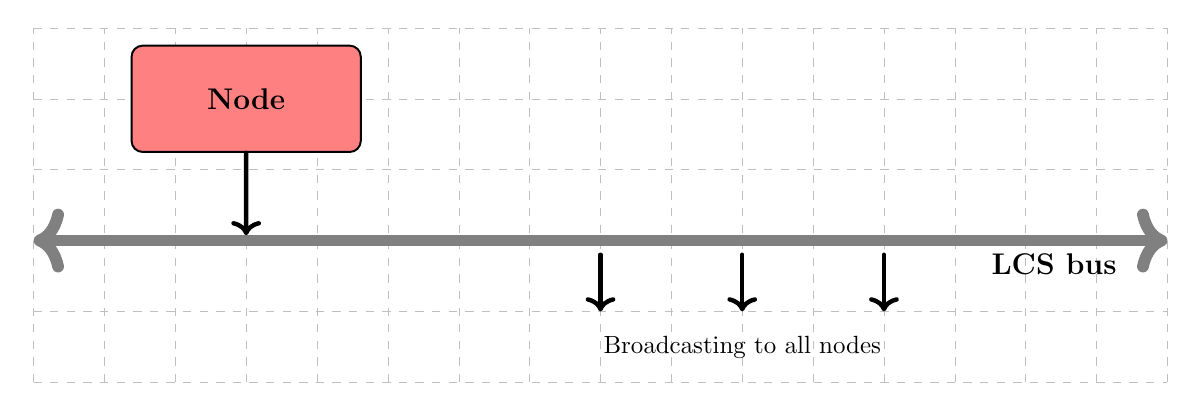
\begin{tikzpicture} [scale=0.9, transform shape]

        \draw[help lines, gray!50, dashed] (0,0) grid(16,5);

         % Thick horizontal line (LCS bus) with text
         \draw[line width=1.5mm, <->, line cap=round, draw=gray, name path=lcsline] 
         (0,2) -- (16,2)
         node[pos= 0.9, tsLargeBold, below] {LCS bus};

          % Define a node
        \node[  tsRoundedRectangle, 
        minimum width=3cm,
        minimum height=1.5cm,
        text width=3cm,
        text centered,
        fill=red!50] (n) at (3,4) {Node};

         % Connecting arrows to LCS bus
        \path[name path=p1] (n.south) -- (3,2); % Define arrow path
        \path[name intersections={of=lcsline and p1, by=intpoint1}];
        \coordinate (adjustedPoint1) at ($(intpoint1) + (0,0.75mm)$);
        \draw[->, ultra thick, line cap=round] (n.south) -- (adjustedPoint1);

        \draw[->, ultra thick, line cap=round] (8, 1.8) -- (8, 1);
        \draw[->, ultra thick, line cap=round] (10, 1.8) -- (10, 1);
        \draw[->, ultra thick, line cap=round] (12, 1.8) -- (12, 1);

        \node at ( 10,0.5) {Broadcasting to all nodes};

    \end{tikzpicture}
\end{center}

All nodes communicate via the layout control bus by broadcasting messages. Every node can send a message, and every node receives the message broadcasted. There is no central master. Since all nodes receive all messages, a node needs to decide whether to react to a message or not. General management and emergency type messages are handled by all nodes. A reply to a specific request will only be handled by the requesting node. The layout control system defines a fairly large set of messages, which can be grouped into several categories:

\begin{smallGapItemize}
    \item General management
    \item Node and Port management
    \item Event management
    \item DCC Track management
    \item DCC Locomotive Decoder management
    \item DCC Accessory Decoder management
    \item RailCom DCC Packet management
    \item Raw DCC Packet management
    \item Firmware Update management
\end{smallGapItemize}

The current implementation is using the CAN bus, which ensures by definition that a message is correctly transmitted. However, it does not guarantee that the receiver actually processed the message. For critical messages, a request-reply scheme is implemented on top. Also, to address possible bus congestion, a priority scheme for messages is implemented to ensure that each message has a chance for being transmitted.

A message is a data packet of up to 8 bytes. The first byte represents the operation code. It encodes the length of the entire packet and opcode number. The first 3 bits represent the length of the message, the remaining 5 bits represent the opCode. For a given message length, there are 32 possible opcode numbers. The last opcode number in each group, 0x1F, is reserved for possible extensions of the opcode number range. The remaining bytes are the data bytes, and there can be zero to seven bytes. 

The message format is independent of the underlying transport method. If the bus technology were replaced, the payload would still be the same. For example, an Ethernet gateway could send those messages via the UDP protocol. The messages often contain 16-bit values. They are stored in two bytes, the most significant byte first and labeled ``xxx-H'' in the message descriptions to come. The message format shown in the tables of this chapter just presents the opCode mnemonic. The actual value can be found in the core library include file.

The byte fields names in an LCS message are explained in greater detail when we discuss the runtime library. For this chapter, the term \texttt{npId-x} will refer to node/port/channel identifier. A node/port/channel identifier is a 16-bit word which consists of the 8-bit nodeId, the 4-bit portId and the 4-bit channel Id. The npId with a portId and channelId of zero will refer to the node itself. The term \texttt{sId} refers to a locomotive session. The remaining message field names, such as \texttt{UID} or \texttt{spDir} or \texttt{argN}are fairly self-explaining.

\section{General Management}

The general management message group contains commands for dealing with the layout system itself. The reset command \texttt{(RESET)} directs all hardware modules, a node, or a port on a node to perform a reset. The entire bus itself can be turned on and off \texttt{(BUS-ON, BUS-OFF)}, enabling or suppressing the message flow. Once the bus is off, all nodes wait for the bus to be turned on again. In case of an emergency the \texttt{(E-STOP)} message stops all running engines. The base station broadcasts a \texttt{(SYS-TIME)} message with the layout time, \texttt{(LCS-INFO)} broadcasts general system information on a regular basis. Finally, there are messages for pinging a node \texttt{(PING)}, perform data synchronization operations \texttt{(SYNC)} and request acknowledgement \texttt{(ACK/ERR)}.

\begin{table}[ht!]
    \centering 
    \resizebox{0.9\textwidth}{!}{ 
        \begin{tabular}{|l|l|l|l|l|l|l|l|}
            \hline
            \textbf{Opcode} & \textbf{Data1} & \textbf{Data2} & \textbf{Data3} & \textbf{Data4} & \textbf{Data5} & \textbf{Data6} & \textbf{Data7} \\
            \hline
            RESET & npId-H & npId-L & flags & & & & \\
            BUS-ON & & & & & & & \\
            BUS-OFF & & & & & & & \\
            E-STOP & & & & & & & \\
            SYS-TIME & arg1 & arg2 & arg3 & arg4 & & & \\
            LCS-INFO & arg1 & arg2 & arg3 & arg4 & & & \\
            PING & npId-H & npId-L & & & & & \\
            ACK & npId-H & npId-L & & & & & \\
            ERR & npId-H & npId-L & code & arg1 & arg2 & & \\
            \hline
        \end{tabular}
    }
\end{table}

\section{Node Id Setup}

When a hardware module is powered on, the first task is to establish the node Id in order to broadcast and receive messages. The \texttt{(REQ-NID)} and \texttt{(REP-ID)} messages are the messages used to implement the protocol for establishing the nodeId. More on this in the chapter on message protocols. A virgin node has the hardware module-specific node type and a node Id of \texttt{NIL} also be set directly through the \texttt{(SET-NID)} command. This is typically done by a configuration tool.

\begin{table}[ht!]
    \centering 
    \resizebox{0.9\textwidth}{!}{ 
        \begin{tabular}{|l|l|l|l|l|l|l|l|}
            \hline
            \textbf{Opcode} & \textbf{Data1} & \textbf{Data2} & \textbf{Data3} & \textbf{Data4} & \textbf{Data5} & \textbf{Data6} & \textbf{Data7} \\
            \hline
            REQ-NID & nId-H & nId-L & nUID-4 & nUID-3 & nUID-2 & nUID-1 & flags \\
            REP-NID & nId-H & nId-L & nUID-4 & nUID-3 & nUID-2 & nUID-1 & flags \\
            SET-NID & nId-H & nId-L & nUID-4 & nUID-3 & nUID-2 & nUID-1 & flags \\
            NCOL    & nId-H & nId-L & nUID-4 & nUID-3 & nUID-2 & nUID-1 & \\
            \hline
        \end{tabular}
    }
\end{table}

All nodes monitor the message flow to detect a potential node collision. This could be for example the case when a node from one layout is installed in another layout. When a node detects a collision, it will broadcast the \texttt{(NCOL)} message and enter a halt state. Manual interaction is required. A node can be restarted with the \texttt{(RES-NODE)} command, given that it still reacts to messages on the bus. All ports on the node will also be initialized. In addition a specific port on a node can be initialized. The hardware module replies with an \texttt{(ACK)} message for a successful node Id and completes the node Id allocation process. As the messages hows, node and port ID are combined. LCS can accommodate up to 4095 nodes, each of which can host up to 15 ports. A Node ID 0 is the NIL node. Depending on the context, a port Id of zero refers all ports on the node or just the node itself.

\section{Node and Port Attributes}

The query node \texttt{(NODE-GET)} and node reply messages \texttt{(NODE-REP)} are available to obtain attribute data from the node or port. The \texttt{(NODE-SET)} allows to set attributes for a node or port for the targeted node. Items are numbers assigned to a data location or an activity. There are reserved items such as getting the number of ports, or setting an LED. In addition, the firmware programmer can also define items with node specific meaning. The firmware programmer defined items are accessible via the \texttt{(NODE-REQ)} and \texttt{(NODE-REP)} messages.

\begin{table}[ht!]
    \centering 
    \resizebox{0.9\textwidth}{!}{ 
        \begin{tabular}{|l|l|l|l|l|l|l|l|}
            \hline
            \textbf{Opcode} & \textbf{Data1} & \textbf{Data2} & \textbf{Data3} & \textbf{Data4} & \textbf{Data5} & \textbf{Data6} & \textbf{Data7} \\
            \hline
            NODE-GET & npId-H & npId-L & item & arg1-H & arg1-L & arg2-H & arg2-L \\
            NODE-SET & npId-H & npId-L & item & val1-H & val1-L & val2-H & val2-L \\
            NODE-REQ & npId-H & npId-L & item & arg1-H & arg1-L & arg2-H & arg2-L \\
            NODE-REP & npId-H & npId-L & item & arg1-H & arg1-L & arg2-H & arg2-L \\
            \hline
        \end{tabular}
    }
\end{table}

Nodes do not react to configuration type messages when in operations mode. To configure a node, the node needs to be put into configuration mode. The \texttt{(OPS)} and \texttt{(CFG)} commands are used to put a node into configuration mode or operation mode. Not all messages are supported in operations mode and vice versa. For example, to set a new nodeId, the node first needs to be put in configuration mode. During configuration mode, no operational messages are processed.

\begin{table}[ht!]
    \centering 
    \resizebox{0.9\textwidth}{!}{ 
        \begin{tabular}{|l|l|l|l|l|l|l|l|}
            \hline
            \textbf{Opcode} & \textbf{Data1} & \textbf{Data2} & \textbf{Data3} & \textbf{Data4} & \textbf{Data5} & \textbf{Data6} & \textbf{Data7} \\
            \hline
            OPS & npId-H & npId-L & & & & & \\
            CFG & npId-H & npId-L & & & & & \\
            \hline
        \end{tabular}
    }
\end{table}

\section{Event Management}

The event management group contains the messages to configure the node event map and messages to broadcast an event and messages to read out event data. The (SET-NODE) with the item value to set and remove an event map entry from the event map is used to manage the event map. An inbound port can register for many events to listen to, and an outbound port will have exactly one event to broadcast. Ports and Events are numbered from 1 onward. When configuring, the portId \texttt{NIL} has a special meaning in that it refers to all portIds on the node.

\begin{table}[ht!]
    \centering 
    \resizebox{0.9\textwidth}{!}{ 
        \begin{tabular}{|l|l|l|l|l|l|l|l|}
            \hline
            \textbf{Opcode} & \textbf{Data1} & \textbf{Data2} & \textbf{Data3} & \textbf{Data4} & \textbf{Data5} & \textbf{Data6} & \textbf{Data7} \\
            \hline
            EVT-ON & npId-H & npId-L & evId-H & evId-L & & & \\
            EVT-OFF & npId-H & npId-L & evId-H & evId-L & & & \\
            EVT & npId-H & npId-L & evId-H & evId-L & arg-H & arg-L & \\
            \hline
        \end{tabular}
    }
\end{table}

\section{DCC Track Management}

Model railroads run on tracks. Imagine that. While on a smaller layout, there is just the track, the track on a larger layout is typically divided into several sections, each controlled by a track node \textnormal{(centralized node or decentralized port)}. The system allows to report back the track sections status \textnormal{(in terms of occupied, free, and detecting the number of engines currently present)}. This function is implemented via the get and set attribute messages. In addition, there are messages to turn on and off the entire tracks.

\begin{table}[ht!]
    \centering 
    \resizebox{0.9\textwidth}{!}{ 
        \begin{tabular}{|l|l|l|l|l|l|l|l|}
            \hline
            \textbf{Opcode} & \textbf{Data1} & \textbf{Data2} & \textbf{Data3} & \textbf{Data4} & \textbf{Data5} & \textbf{Data6} & \textbf{Data7} \\
            \hline
            TON & npId-H & npId-L & & & & & \\
            TOF & npId-H & npId-L & & & & & \\
            \hline
        \end{tabular}
    }
\end{table}

\section{DCC Locomotive Decoder Management}

Locomotive management comprises the set of messages that the base station uses to control the running equipment. To control a locomotive, a session needs to be established \texttt{(REQ-LOC)}. This command is typically sent by a cab handheld and handled by the base station. The base station allocates a session and replies with the \texttt{(REP-LOC)} message that contains the initial settings for the locomotive speed and direction. \text{(REL-LOC)} closes a previously allocated session. The base station answers with the \texttt{(REP-LOC)} message. The data for an existing DCC session can requested with the \texttt{(QRY-LOC)} command. Data about a locomotive in a consist is obtained with the \texttt{(QRY-LCON)} command. In both cases the base station answers with the \texttt{(REP-LOC)} message.

\begin{table}[ht!]
    \centering 
    \resizebox{0.9\textwidth}{!}{ 
        \begin{tabular}{|l|l|l|l|l|l|l|l|}
            \hline
            \textbf{Opcode} & \textbf{Data1} & \textbf{Data2} & \textbf{Data3} & \textbf{Data4} & \textbf{Data5} & \textbf{Data6} & \textbf{Data7} \\
            \hline
            REQ-LOC & adr-H & adr-L & flags & & & & \\
            REP-LOC & sId & adr-H & adr-L & spDir & fn1 & fn2 & fn3 \\
            REL-LOC & sId & & & & & & \\
            QRY-LOC & sId & & & & & & \\
            QRY-LCON & conId & index & & & & & \\
            \hline
        \end{tabular}
    }
\end{table}

Once the locomotive session is established, the \texttt{(SET-LSPD)}, \texttt{(SET-LMOD)}, \texttt{(SET-LFON)}, \texttt{(SET-LOF)} and \texttt{(SET-FGRP)} are the commands sent by a cab handheld and executed by the base station to control the locomotive speed, direction and functions. \texttt{(SET-LCON)} deals with the locomotive consist management and \texttt{(KEEP)} is sent periodically to indicate that the session is still alive. The locomotive session management is explained in more detail in a later chapter when we talk about the base station.

\begin{table}[ht!]
    \centering 
    \resizebox{0.9\textwidth}{!}{ 
        \begin{tabular}{|l|l|l|l|l|l|l|l|}
            \hline
            \textbf{Opcode} & \textbf{Data1} & \textbf{Data2} & \textbf{Data3} & \textbf{Data4} & \textbf{Data5} & \textbf{Data6} & \textbf{Data7} \\
            \hline
            SET-LSPD & sId & spDir & & & & & \\
            SET-LMOD & sId & flags & & & & & \\
            SET-LFON & sId & fNum  & & & & & \\
            SET-LFOF & sId & fNum  & & & & & \\
            SET-FGRP & sId & fGrp  & data & & & & \\
            SET-LCON & sId & conId & flags & & & & \\
            KEEP & sId & & & & & & \\
            \bottomrule
        \end{tabular}
    }
\end{table}

Locomotive decoders contain configuration variables too. They are called CV variables. The base station node supports the decoder CV programming on a dedicated track with the \texttt{(REQ-CVS)}, \texttt{(REP-CVS)} and \texttt{(SET-CVS)} messages. The \texttt{(SET-CVM)} message supports setting a CV while the engine is on the main track. \texttt{(DCC-ERR)} is returned when an invalid operation is detected.

\begin{table}[ht!]
    \centering 
    \resizebox{0.9\textwidth}{!}{ 
        \begin{tabular}{|l|l|l|l|l|l|l|l|}
            \hline
            \textbf{Opcode} & \textbf{Data1} & \textbf{Data2} & \textbf{Data3} & \textbf{Data4} & \textbf{Data5} & \textbf{Data6} & \textbf{Data7} \\
            \hline
            SET-LSPD & sId & cv-H & cv-L & mode & val & & \\
            REQ-CVS  & cv-H & cv-L & mode & val & & & \\
            REP-CVS  & cv-H & cv-L & val  & & & & \\
            SET-CVS  & cv-H & cv-L & mode & val & & & \\
            \hline
        \end{tabular}
    }    
\end{table}

The SET-CVM command allows to write to a decoder CV while the decoder is on the main track. Without the RailCom channel, CVs can be set but there is not way to validate that the operation was successful.

\section{DCC Accessory Decoder Management}

Besides locomotives, the DCC standards defines stationary decoders, called accessories. An example is a decoder for setting a turnout or signal. There is a basic and an extended format. The \texttt{(SET-BACC)} and \texttt{(SET-EACC)} command will send the DCC packets for stationary decoders. Similar to the mobile decoders, there are POM / XPOM messages to access the stationary decoder via RailCom capabilities.

\begin{table}[ht!]
    \centering 
    \resizebox{0.9\textwidth}{!}{ 
        \begin{tabular}{|l|l|l|l|l|l|l|l|}
            \hline
            \textbf{Opcode} & \textbf{Data1} & \textbf{Data2} & \textbf{Data3} & \textbf{Data4} & \textbf{Data5} & \textbf{Data6} & \textbf{Data7} \\
            \hline
            SET-BACC & adr-H & adr-L & flags & & & & \\
            SET-EACC & adr-H & adr-L & val & & & & \\
            \hline
        \end{tabular}
    }
\end{table}

These commands are there for completeness of the DCC control interfaces. There could be devices that are connected via the DCC track that we need to support. However, in a layout control system the setting of turnouts, signals and other accessory devices are more likely handled via the layout control bus messages and not via DCC packets to the track. This way, there is more bandwidth for locomotive decoder DCC packets.

\section{RailCom DCC Packet management}

With the introduction of the RailCom communication channel, the decoder can also send data back to a base station. The DCC POM and XPOM packets can now not only write data but also read out decoder data via the RailCom back channel. The following messages allow to send the POM / XPOM DCC packets and get their RailCom based replies.

\begin{table}[ht!]
    \centering 
    \resizebox{0.9\textwidth}{!}{ 
        \begin{tabular}{|l|l|l|l|l|l|l|l|}
            \hline
            \textbf{Opcode} & \textbf{Data1} & \textbf{Data2} & \textbf{Data3} & \textbf{Data4} & \textbf{Data5} & \textbf{Data6} & \textbf{Data7} \\
            \hline
            SET-MPOM & sId & ctrl & arg1 & arg2 & arg3 & arg4 & \\
            REQ-MPOM & sId & ctrl & arg1 & arg2 & arg3 & arg4 & \\
            REP-MPOM & sId & ctrl & arg1 & arg2 & arg3 & arg4 & \\
            SET-APOM & adr-H & adr-L & ctrl & arg1 & arg2 & arg3 & arg4 \\
            REQ-APOM & adr-H & adr-L & ctrl & arg1 & arg2 & arg3 & arg4 \\
            REP-APOM & adr-H & adr-L & ctrl & arg1 & arg2 & arg3 & arg4 \\
            \hline
        \end{tabular}
    }
\end{table}

The XPOM messages are DCC messages that are larger than what a CAN bus packet can hold. With the introduction of DCC-A such a packet can hold up to 15 bytes. The LCS messages therefore are sent in chunks with a frame sequence number and it is the responsibility of the receiving node to combine the chunks to the larger DCC packet.

\section{Raw DCC Packet Management}

The base station allows to send raw DCC packets to the track. The \texttt{(SEND-DCC3)}, \texttt{(SEND-DCC4)}, \texttt{(SEND-DCC5)} and \texttt{(SEND-DCC6)} are the messages to send these packets. Any node can broadcast such a message, the base station is the target for these messages and will just send them without further checking. So you better put the DCC standard document under your pillow.

\begin{table}[ht!]
    \centering 
    \resizebox{0.9\textwidth}{!}{ 
        \begin{tabular}{|l|l|l|l|l|l|l|l|}
            \hline
            \textbf{Opcode} & \textbf{Data1} & \textbf{Data2} & \textbf{Data3} & \textbf{Data4} & \textbf{Data5} & \textbf{Data6} & \textbf{Data7} \\
            \hline
            SEND-DCC3 & arg1 & arg2 & arg3 & & & & \\
            SEND-DCC4 & arg1 & arg2 & arg3 & arg4 & & & \\
            SEND-DCC5 & arg1 & arg2 & arg3 & arg4 & arg5 & & \\
            SEND-DCC6 & arg1 & arg2 & arg3 & arg4 & arg5 & arg6 & \\
            \hline
        \end{tabular}
    }
\end{table}

The above messages can send a packet with up to six bytes. With the evolving DCC standard, larger messages have been defined. The XPOM DCC messages are a good example. To send such a large DCC packet, it is decomposed into up to four LCS messages. The base station will assemble the DCC packet and then send it. 

\begin{table}[ht!]
    \centering 
    \resizebox{0.9\textwidth}{!}{ 
        \begin{tabular}{|l|l|l|l|l|l|l|l|}
            \hline
            \textbf{Opcode} & \textbf{Data1} & \textbf{Data2} & \textbf{Data3} & \textbf{Data4} & \textbf{Data5} & \textbf{Data6} & \textbf{Data7} \\
            \hline
            SEND-DCCM & ctrl & arg1 & arg2 & arg3 & arg4 & & \\
            \hline
        \end{tabular}
    }
\end{table}

\section{DCC errors and status}

Some DCC commands return an acknowledgment or an error for the outcome of a DCC subsystem request. The \texttt{(DCC-ACK)} and \texttt{(DCC-ERR)} messages are defined for this purpose.

\begin{table}[ht!]
    \centering 
    \resizebox{0.9\textwidth}{!}{ 
        \begin{tabular}{|l|l|l|l|l|l|l|l|}
            \hline
            \textbf{Opcode} & \textbf{Data1} & \textbf{Data2} & \textbf{Data3} & \textbf{Data4} & \textbf{Data5} & \textbf{Data6} & \textbf{Data7} \\
            \hline
            DCC-ACK & & & & & & & \\
            DCC-ERR & code & arg1 & arg2 & & & & \\
            \hline
        \end{tabular}
    }
\end{table}

\section{Analog Engines}

The messages defined for the DCC locomotive session management as outlined above are also used for the analog engines. An analog engine will just like its digital counterpart have an allocated locomotive session and the speed/dir command is supported. All other commands will of course not be applicable. The speed/dir command will be sent out on the bus and whoever is in control of the track section where the analog engine is supposed to be, will manage that locomotive. In the following chapters we will answer the question of how exactly multiple analog engines can run on a layout.

\section{Firmware Update Management}

LCS supports a method for updating the firmware remotely. This involves loading a new firmware image. A typical approach is to split the available program memory in two partitions and load the new image in the non-active partition. When the firmware is transmitted and valid, the next restart will boot using the new firmware. There is a whole chapter later in the book about the firmware update.

\begin{table}[ht!]
    \centering 
    \resizebox{0.9\textwidth}{!}{ 
        \begin{tabular}{|l|l|l|l|l|l|l|l|}
            \hline
            \textbf{Opcode} & \textbf{Data1} & \textbf{Data2} & \textbf{Data3} & \textbf{Data4} & \textbf{Data5} & \textbf{Data6} & \textbf{Data7} \\
            \hline
            START-LOAD & npId-H & npId-L & cmd & size-1 & size-2 & size-3 & size-4 \\
            START-BLOCK & npId-H & npId-L & cmd & blockId-H & blockId-L & & \\
            SEND-DATA & npId-H & npId-L & cmd & data1 & data2 & data3 & data4 \\
            END-BLOCK & npId-H & npId-L & cmd & blockId-H & blockId-L & chkSum-H & chkSum-L \\
            END-LOAD & npId-H & npId-L & cmd & chkSum-1 & chkSum-2 & chkSum-3 & chkSum-4 \\
            \hline
        \end{tabular}
    }
\end{table}

A firmware update starts with the \texttt{(START-LOAD)} message. The transfer uses the \texttt{(START-BLOCK)}, \texttt{(SEND-DATA)} and \texttt{(END-BLOCK)} messages to transmit a block. Each block is validated with a 16-bit checksum. The \texttt{(END-LOAD)} message completes the download, the entire image is checked against a 32-bit checksum.


\section{Summary}

This chapter introduced the general message formats for the layout control bus functions and how they are used in the LCS protocols. The message format is built upon an 8-byte message format that is suitable for the industry standard CAN bus. Although there are many other standards and communication protocols, the CAN bus is a widely used and robust bus. Since all data is encoded in the message, there is no reason to select another communication media. But right now, it is CAN. The next chapter will now concentrate on the message protocols.
 
    \include{chapters/chapter-lcs-concepts-message-protocols} 
    \include{chapters/chapter-lcs-concepts-dcc-subsystem}
    \include{chapters/chapter-lcs-concepts-analog-subsystem}
    \chapter{Hardware Modules}

talk a little about the modules and extensions ...

we will have a main board and extension boards

main board hosts the controller and perhaps special HW that needs to be close to the controller

they will always have the LCS bus interface and a power supply for itself and the extentions

extensions are access via a I2C bus

they implement functions for as sensors and actors

there is a standardized interface connector between main board and extension boards

up to 4 extension boards can be connected to a main board




    \chapter{Sensors and Actors}

Sensors and Actors are the eyes, ears and hands for any layout system. The requirements and options are numerous and the list of desired features needed is perhaps never complete. Sensors, the eyes and ears, are mainly the event producers. A block occupancy detection, a power overload detection, but also a push of a button on a layout control panel are good examples. The counterpart to sensors  are actors. Actors, the hands, are the family of LCS nodes and special hardware that control turnouts, signals and whatever else there is. This chapter will present the most common actors and sensor nodes found on a layout. Building upon the concept of main controller, base station, block controller and extensions board concepts, this part of the book will present how the pieces that make up a node can be put together from the basic building blocks.

With so many sensors and actors, a key requirement is to implement a concept where most of the functional parts can be used in different combinations. The chapter on hardware design already presented the main controller and extensions concept. A key reason for this concept were exactly the large variety of sensors and actors.

\begin{itemize}
\item main controller
\item block controller
\item base station
\end{itemize}

The main controller portion, common to all, will feature the processor, the message interface for the LCS bus, and the power supply for the board and the extensions. Some LCS nodes need a larger NVM storage. The main controller board will allow an optional installation of a NVM chip. Furthermore, the power supply, intended for generating the power for main controller board as well as the VCC power for the extensions, will also feature an optional installation of power failure detection. Before going into the detailed extension board designs, what boards would be need? Here is a brief look ahead of the boards to come.
\begin{itemize}
\item \textbf{Occupancy Detector}. The occupancy detector extension board is a companion to the block controller board. It will offer 4 channels, i.e. tracks that match the block controller output, with a set of detectors on each channel.
\item \textbf{Turnout}. The turnout extension board features a set of turnouts with frog polarization. Similar to the occupancy detector the boards is designed to go with the block controller board.
\item \textbf{Servo}. The servo extension board is a universal board, which can be connected to any controller board presented. It features a set of general servo outputs.
\item \textbf{GPIO}. The GPIO extension boards is a universal digital input / output board. It is typically used for input such as switches or push buttons a well as LEDs connected. Care has to be taken to match the the number of output consumers with the what the individual output pins can drive.
\item \textbf{Signal}. The signal extension bard is another general purpose board designed for driving the LED equipped signals. It is able to not only match the power requirements but also allow for dimming and / or blinking the individual lights.
\item \textbf{Relays}. The relay extension board is a general purpose board intended to drive a set of relays. The relays, which are not part of the board, can be driven with different voltage levels.
\item \textbf{Cab Control}. The cab handhelds as well as stationary cab control devices are also just an extension. There is no reason why this extension could for example not be connected to a base station and build a complete control station fort a smaller layout.
\item \textbf{Prototyping}. It is often useful to just do a quick sketch of a function desired for an extension board. So, how about an extension board with the extension address resolution logic and just room for building your own HW designs.
\end{itemize}

Extension boards implements the hardware for the particular sensor or actor type. All extension boards need to feature the connectors, so that more than one extension board can share the same controller board. However, only the first board will benefit from the availability of all extension bus signal lines. It is not a requirement that the second extension board will get the same signals. It is also not a requirement that an extension board does have the decoding logic described in the extension hardware design chapter. For example, the power module unit which together with main controller is a base station, does not have that logic. It expects to be connected directly to the main controller board. The power module board will however still route power, DCC and I2C signals. The I2C bus plays a key role in communicating with an I2C type extension board. Each I2C based extension board will have the extension board decoding logic, which is essential for proper addressing that board.
    \include{chapters/chapter-lcs-concepts-summary}

    %----------------------------------------------------------------------------
    \part{LCS Core Layer} 
    
    \include{chapters/chapter-lcs-runtime-lib}
    \include{chapters/chapter-lcs-runtime-lib-command-interface}
    %-------------------------------------------------------------------------------------------------------
%
%-------------------------------------------------------------------------------------------------------
\chapter{ RtLib Usage Example}

??? what is a good comprehensive example ?

??? a simple button to push and a LED to light up. show attributes, requests, callbacks, events.

??? use the commands to show what is stored where...

??? use the diagnostic program to show how to write a program and at the same show how we actually test the runtime. 
    \include{chapters/chapter-lcs-controller-dependent-code} 
    \include{chapters/chapter-lcs-ui-elements}
    \chapter{LCS Node Firmware Design}

The previous chapters introduced the overall Layout Control System architecture, the communication concepts and how an LCS node could be implemented. The hardware design chapter also presented the main controller and extension concept for splitting up the work between the generic controller and a specific extension. We are about to embark on designing specific LCS nodes such as a base station or a block controller. Before we do that, this chapter will outline how in general one does write firmware for the layout control system. This chapter will not focus on the how to use the library. This was explained before in small examples, and the major modules firmware code to follow in the next chapters contains good larger examples for firmware designs. This chapter will rather focus on how you go about designing a firmware for a node and give guidelines and recommendations.

\section{General Thoughts - Nodes, Ports and Events}

It is the general philosophy of any software system to find a good balance between what is coded or written in firmware and what is done with setting configuration values. Without a concept how to enter configuration values, even a simple change would result in downloading the firmware with the changed data. Clearly, we need a better way. The idea should be to update the firmware only when there are new features, fixes to bugs, and new installations of hardware capabilities of the node. This first of all means that each hardware capability is accessible through user defined port and node control and info items. That was a key reason why there is a range if user definable items for these attributes. A configuration system can query and set defined attributes and also execute functions mapped behind a node or port item.

Just using the ability to send messages to a node and port allows already for a very capable control system. Similar to the DCC CV variables, nodes and ports have a set of variables that can be queried and modified form any node. The addition of callbacks in the path of accessing such a variable, allows to implement for example querying a hardware resource and return the result via the variable associated with it. In addition, the firmware designer can define custom items that will invoke a callback function. This function now can do all kind of things. It is completely up to the firmware designer what this function will do on that node. Just using the node and port item concept, a control system could be implemented with a central station containing buttons, switches and status LEDs that send these messages to node which then set the turnout direction acknowledgement, which in turn set the LED. This way we know the turnout direction setting. A central concept, but with few wires. Only the bus lines go across the layout. But that alone would just mean a more economic wiring approach. And the central bus bus load would perhaps be considerable for larger layouts. A CAN bus frame is between 58 and 114 bits. With a baud rate of 500Kbits and an assumed average packet length of 6 bytes, roughly 5000 frames per second are the limit.

The addition of an eventing system allows for all nodes to react on events broadcasted by any other node. A setting of a turnout, for example, could result in broadcasting an event for all other nodes to see. The central station mentioned before could use this event to set an LED light on the control panel to show the turnout setting. Instead of periodically polling the turnout setting, we now just process the respective event. Furthermore, since all nodes can see all events, many nodes can react to an event sent. All that needs to be done is to configure the port to react on the given event though invoking a callback. Events provide a great flexibility on top of the query and set scheme outlined before.

Let's take the common example of setting a route. This would involve a node where there is some button or other way to broadcast the "set route" event. Each node that has a turnout belonging to the route was configured to act on this event and the port representing the turnout would then take action via the callback. A simple "event delay" capability allows to set one turnout after the other and not all at once. The nice thing about the event driven approach is that the ports need not be on the same node. And, more importantly, the callback functions are just controlling a piece of hardware and the need for updating the node firmware would only be needed for entire new capabilities, firmware update or bug correction. In short, there is a fine line with what the firmware should do and what is delegated to configuring ports and events.

It would be tempting to also offer a kind of macro capability to execute a macro instead of actual code. Upon receiving an event, the macro would be executed. And going this route we are just about to invent yet another language. Right now, the jury is out whether this is really required. The whole philosophy of the Layout Control system is that events are produced and visible for all nodes and each port on a node can act on this event. Node local processing just concerns the sensors and actors belonging to that node. If on a node more than one port is registered for an event the ports are triggered in ascending order. It really depends what the callback functions associated with the port are executing.

\section{General thoughts - Software layers}

The layout control system will over time contain many hardware and software components. The software therefore needs to be structured in a way that the firmware designer just will focus on the the tasks at hand and all else is being taken care of by the core library. Well, almost. The great variety of hardware requires a slightly more detailed picture.

\begin{center}
    \begin{tikzpicture}[scale=0.9, transform shape]
        
        \draw[help lines, gray!50, dashed] (0,0) grid(16,8);
        \node at (8,4) {Runtime Lib refined};
    \end{tikzpicture}
\end{center}

Besides whatever the node is designed for, there are the common firmware layers. It all starts with the \textbf{controller dependent code}, that shields the actual controller family from the rest of the library. This does not mean that any special hardware feature of the controller is not available it just means that the common capabilities to be found across the implementations are available via a common layer. Examples are the routines to mange a digital I/O pin, the analog input, hardware timers and so on. The \textbf{non-volatile memory} CDC library part implements a simple memory that is used by the node firmware but also the firmware designer. Some controllers do have a non volatile memory area, often an EEPROM, others don't. The library offers a simple abstraction for storing non volatile data. The \textbf{ CAN Bus} CDC library part is responsible for implementing the CAN bus interface, which is either implemented as a separate hardware chip or implemented in software using the controller special capabilities, such as the Raspberry Pi Pico programmable IO blocks.

At the heart of all node specific firmware is the \textbf{LCS node library}. It itself uses the aforementioned CDC libraries where needed. The LCS library actually implements the event loop where events and message are handled and manages the node data. Any firmware written for a node sits on top of this library, but still has access to the underlaying hardware. 

Extension boards need their own piece of software to manage whatever the extension board implements. We will call this a \textbf{extension driver}. A driver is access using a defined set of routines available through the node library. Firmware programmers think of such a board as a peripheral device that is access though a set of control, info, read and write functions. The core library contains a set of functions to manage the driver subsystem. Examples are extension board discovery and address mapping.

... mapped to ports....

Finally, there is the \textbf{node specific firmware}. This part is written by the firmware designer, i.e. you. It communicates with the lower layers through the set of defined APIs and the set of defined callbacks. In fact, a great deal of firmware specific code development is just writing the callback handlers for the core library and calls to the respective extension driver API.  The main routine of a node just consists of call to initialize the library, registers the callbacks and let the library loop do its work. Throughout the chapters that implement specific nodes, you will see this basic structure.

\section{Node Functions and Attributes}

A key idea of designing the firmware is that there is no need to update the firmware every time configuration or other parameters change. It is in a sense quite similar to a DCC decoder which offers a large set of variables that can be set with values that the decoder firmware interprets. LCS nodes have a concept of attributes that is very similar to these variables. A node variable can be queried and set from any other node.

Node variables are accessed via "items". An item is just a number that refers to the variable. Besides a set of fixed, i.e. reserved, items that the system itself offers, a set of items allow to access a variable in memory or NVM. Any values that you want to keep across a power cycle can be stored in these variables. The idea is that during startup the values are simply copied form NVM to memory for usage. In the opposite way, there is a set of items that when used, will store a new value in memory and NVM. So, while the memory value can change quite a bit during operation, startup always used a known fixed value.

A node has up to 128 such variables. That is not a lot, you might say. Well, not quite. The item range has a set of 64 user definable items. These are items that when accessed will result in a callback to the node firmware. And in such a callback function, you can do anything you like, including accessing these local attributes of course. Beyond this way of using a user definable callback, these callbacks offers a very flexible to directly access firmware functions without going through kludges of writing a value to a variable that is interpreted as a functions. Since accessing local attributes is such a common scenario, you will find in the reserved item section also items that allows to directly read and write to local attributes.

Finally, think about where these variable values would come from. There will be the day where a hardware piece breaks down and needs to be restored. It is rather easy to load the node variables and attributes from a central database, as well as to first of all store these values in such a place.

\section{Port Functions and Attributes}

Ports are the higher level endpoints on a node. They too features variables accessible via the items already presented. There are just no local attributes related to a port. But what is a port actually used for? When designing a node firmware, the designer should use ports to group functions that are accessible by a combination of node and port identifiers. As seen in the concepts chapter, they together form a 16-bit value. A good example is a block controller that has four channels to manage a block on the layout. Each block, you guessed it, can be represented as a port. When talking to the block, just the node and port ID is enough to address it.

... idea of a path to describe an element in an extension board. We would need for example to access the state of sections in a block, a single section and also the state of all sections.

... node:port:element is a path. ( where port is one of the driver mapped ports )

... driver code just needs to deal with port:element locally

... elements are accessed via the GET/PUT/REQ items defined. 

... what exactly can be accessed from other notes ?

.. rough idea:

\lstset{language=c++, style=codesnippetstyle}
\begin{lstlisting}
   
    union pathDesc { 

        struct path {

            uint reserved   : 4;
            uint port       : 4;
            uint element    : 8;
        };

        uint16_t word;
    }
    
\end{lstlisting}


But ports are also the endpoint for events. Remember each node can broadcast an event observable by all nodes on the system. Events are created to represent an, well, event that somebody would be interested in. For example a track power shortage. Or a block section is occupied event. Or whatever you see as a reasonable event to broadcast to the world. And again these the event map data can be queried and loaded from another node.

When configuring a node, that node can register its interest in an event by adding an event ID / port ID combo to the event map. How to do this? Well, there is a reserved item function to just do that. A matching incoming event will result in a callback registered for the port. A node offers up to 15 ports. Since they also serve as a logical grouping of physical things on the layout, having 15 ports is a good compromise between number and resources needed by a port. When designing a firmware, the first thinking should be what a node manages and what ports will mange portions controlled by that node.

first four ports map to extensions, port zero to the node.

Attributes work from MEM, when in CFG then NVM is also used.

when in OPS, items SYNC-MEM and SYNC-NVM are used to also update the counterpart.

\section{Command Line and Display}

The LCS library already offers a command line interface. It provides commands for the basic commands to manage a node and access its data. This interface, while not used in regular operation, is very useful for node firmware testing and debugging. All commands are also available via LCS messages, so that troubleshooting and monitoring can be done when the node is already installed. Following this philosophy, implementing node specific commands are a good idea. Writing your own serial commands is just writing a command line callback and registering it at node startup.

\section{Event handling}

The layout control system is an event driven system. A large part of layout configuration consist of creating an event Id, i.e. picking a number, and associating a port with the event. Upon event detection, the port callback is invoked. Configuration is therefore just entering the event/port pair in the node event table. The other direction, a situation at the node results in broadcasting an event, requires that the event ID is known. A good practice is to define port or node attributes that contain the event Id to use. This attribute can be set during node configuration. The LCS core library offers a periodic callback where the firmware designer can implement to manage the local sensor hardware data and decide to broadcast an event.

tbd: how are events handled when the port is driver mapped ?

\section{Periodic Tasks}

Since the core library implement the outer loop, tasks that need to run periodically need to be implemented as callback for the core library to invoke. As always, one can write timer code and management outside of the core library, but this comes at the expense of being dependent on a particular controller hardware. For most cases, a simple callback, it does net even have to be precise to the microsecond, is sufficient. A good example is the checking for power consumption on a track. A firmware designer would provide a callback that is invoked periodically and would make use of the driver interface to obtain the actual data. If the the consumption is outside defined bounds, an event owl  due raised and the track turned ff. 

\section{Extension Board Driver Function}

Driver requests are handled via GET/PUT/REQ calls to the mapped port 1 .. 4.

Concept of a path: \texttt{<node>:<port>:<channel>}

A driver is just the REQ function. 

GET/PUT mapped directly to what a port can do. Common items, attribute items. 

Startup order is INIT, REGISTER, START 



\section{Configuration}

Configuration comes in two parts. There are all the items that need to be handled of ramping the hardware actually perform, and there are the items that are at the higher level of configuring a node for its purpose. A great of how to configure the hardware was already presented in the chapter on the CDC layer. At this layer the hardware setup was place and all capabilities are setup to be used. As a firmware designer, unless you directly access hardware, you may not have to go that deep, the CDC library / Core library will have the configuration data that maps the actual hardware. 

... text ... rework ...

What is left is from a low level perspective are the extension boards and their inner workings. These concepts will be explained in great detail in the chapter on the extension board designs. Right now it is sufficient to know that using the driver interface, some setup and configuration needs to be implemented. For example, setting an I/O pin on a GPIO extension board to be an output port, is a typical configuration task. Again, more on this later.

What is left is the high level configuration, which means to set node and port attributes. This task is comparable to a DCC locomotive decoder. It is has tons of variables  that can be set. The firmware designer is responsible to make all relevant items of the node firmware configurable by exporting them as node and port attributes. When w look at the first larger node example, the base station, this concept becomes clearer.

\section{The main code}

The main code is just a set of firmware specific code and callback routines that do the firmware specific work. During initialization, register the necessary callbacks and then delegate control to the LCS loop. This scheme is common to all nodes. For smaller nodes, the setup code and callback routines can be all in one file, for example the "main.cpp" file. Larger node firmware will perhaps split the code into several files. The \texttt{C++} classes or structures are a good way of structuring your code. There is one caveat though. Callbacks are technically just procedure labels and need to be at either the main code, the file local portion of a separate file or a static methods in a C++ class. In other words, they cannot be object instance methods.

\section{Summary}

This chapter gave a brief overview how one would go after writing node firmware. In short it is writing functions that can be registered as callbacks to the core library and that will in turn use the core library functions for implementing their purpose. It also introduced a more detailed picture of the overall software layers. The heavy lifting of message handling, event handling, node data management, extension board management and overall processing is handled by the LCS library. All the firmware programmer has to do is to write the node and specific functions. 

The appendix contains a reference where all the hardware and software components can be found on \textbf{GitHub}. The source code contains many comments and further explanations. Finally, there are also further references to reading material and related projects.

The following chapters will give several examples of how the firmware for the common nodes such as a base station, a cab handheld and a block controller is designed using the principles and guidelines mentioned in this chapter.


    
    %----------------------------------------------------------------------------
    \part{LCS Hardware}
    
    \include{chapters/chapter-lcs-concepts-hardware-main-module-design}
    \include{chapters/chapter-lcs-main-controller-hardware-pico}
	\include{chapters/chapter-lcs-power-module-design}
    \include{chapters/chapter-lcs-railcom-signal-detector}
    \include{chapters/chapter-lcs-hardware-part-summary}
   
    %----------------------------------------------------------------------------
	\part{LCS Modules}

	\chapter*{The Base Station}
\addcontentsline{toc}{chapter}{The Base Station}

Take a deep breath. Over the next chapters we are about to put together our first major LCS hardware module. The previous chapters introduced the message format and protocols and the core library for implementing the event system as well as the running equipment based on the DCC signal standards. Next, we took a closer look on the major hardware building blocks and power module designs. Just like the LCS core library allows to build a node specific firmware on top, the hardware building blocks are the foundation to build the required hardware modules. We also looked at how one would go after designing the node firmware in general. So here is the first and most important hardware module putting it all together. The base station. Every layout needs to have some kind of a base station that acts as the central place for layout control and signal generation.

Looking at the market, there are plenty of so called base stations. They typically offer support for several standards and communication protocols, such as DCC, mfx, LocoNet, a Can Bus, a S88 sensor bus, and so on. Most base station also have the power module directly integrated. They support the configuration of locomotive and stationary decoders. In short, a one stop all round solution. Their price range is around few hundred Euros. With the advent of Arduino, Raspberry and other controllers there are numerous do it yourself solutions. Just to name one, the \texttt{DCC++} Arduino base station with a motor shield as a power unit, gets you a base station for well under hundred Euros. The excellent work of the JMRI community to provide a \texttt{DCC++} interface for configuration software and other utilities to use this inexpensive base station hardware. The DCC-EX group extended and stabilized the original \texttt{DCC++} work for a wider range of controllers but also with new capabilities. There are many such great projects. The appendix provides some links and pointers to this work.

Our base station needs to deliver the following capabilities. At first it needs to be able to assemble the DCC packets and generate the respective DCC hardware signals. This work is split into the base station producing the signal content and the power section driving the hardware. Furthermore, the base station needs to provide a way to manage several locomotive sessions. For each active session the current state of the locomotive is maintained and the DCC packets are produced. When a new locomotive session is established, a dictionary of locomotives could be consulted about the particular locomotive to get the initial function settings, and so on.

A base station implementing locomotive session and track management should also implement a serial command interface for managing a session or sending commands to a locomotive. Although not really necessary, it is very beneficial for testing and debugging. But also, programming DCC decoders will need some form of getting the configuration data to the decoder. There are great openSource tools out there which make use of an ASCII interface to send their commands. An example is DecoderPro from the JMRI teams. It features among other protocols the \texttt{DCC++} ASCII interface to send and receive commands. Our base station will therefore implement the relevant \texttt{DCC++} commands.

All configuration settings, such as the number of concurrent sessions or the current consumption limit for a track, should be available as attributes on the node itself and ports. A track should be represented by a port, so there will be a port for controlling the MAIN track output, and a port for controlling the PROG tack output.

Finally, the firmware for the base station could also host LCS management functions, such as a configuration database or display data about layout operations. This is not per se a function of the base station, but as each layout needs to have a base station and perhaps display high level status data, it is a convenient place to put central functionality there as well. This subject will be discussed in another chapter, this chapter will focus on the core base station features.


 	\chapter*{Base Station Hardware}
\addcontentsline{toc}{chapter}{Base Station Hardware}

The base station is essentially based on a main controller board and a dual power module unit shown in previous chapters. We will use the PICO controller version and the dual H-Bridge building block. Add the RailCom detectors and stir the whole soup for a while. The extension connector of the base station would still export the I2C interface and the DCC signal produced by the base station. So, adding an I2C based extension board for display, switches, etc. is of course still possible. Here is the schematic for the base station. The individual building blocks should be familiar by now. The first page shows the main controller parts. Note that it needs fewer level shifters, as most of the signals are consumed internal to the board.

\begin{figure}[htbp]
    \centering
    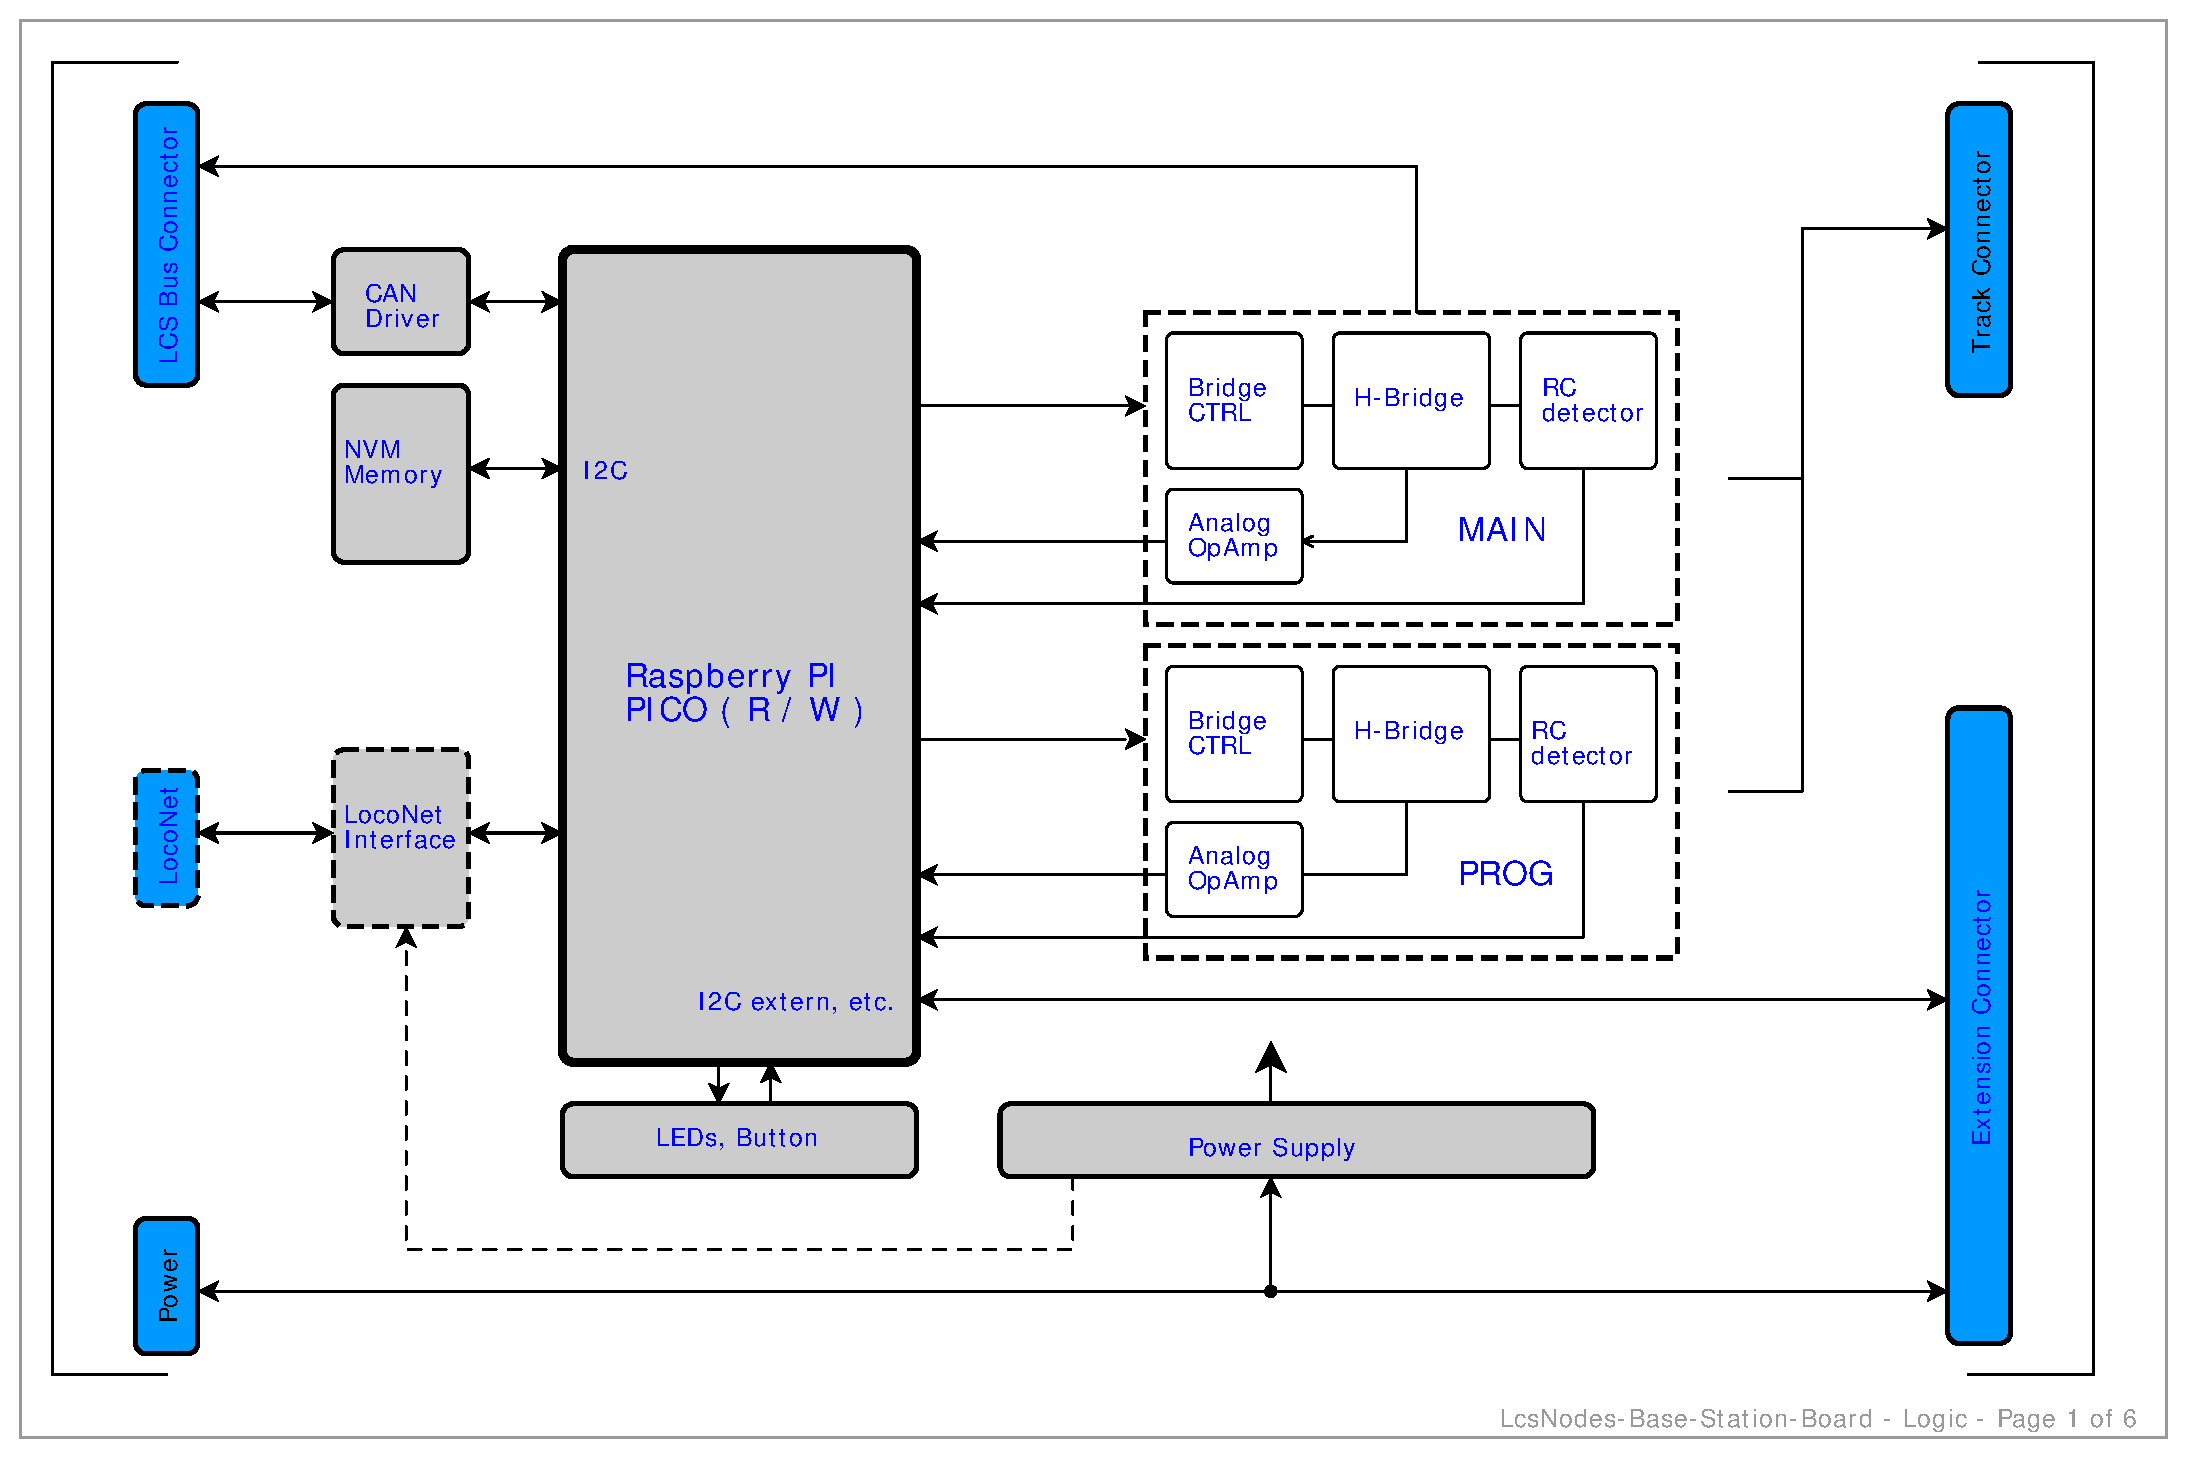
\includegraphics[page=1, width=0.9\textwidth]{schematics/Schematic_LcsNodes-Base-Station-Board.pdf}
    \caption{Base Station Block Diagram}
    %\label{fig:BlockDiagram}
\end{figure}
%\FloatBarrier

\section*{Base Station Main Controller}
\addcontentsline{toc}{section}{Base Station Main Controller}

The Raspberry PI Pico has enough capacity to implement the CAN bus protocol directly using one of the cores. As a result, only the line driver is necessary to implement the CAN bus interface. There are the level shifters for the I2C bus and a few other external signals. The Power supply needs to have a method to detect that there is an USB cable connected to the PICO and ensure that there is no conflict between the power sources. Like any LCS node, the controller needs a non-volatile memory. The base station hosts an I2C type NVM with up to 64Kbytes. The key reason for such a high capacity is that a base station might store a lot of data for each engine that it can manage.

\begin{figure}[htbp]
    \centering
    \includegraphics[page=2, width=0.9\textwidth]{schematics/Schematic_LcsNodes-Base-Station-Board.pdf}
    \caption{Base Station Main Controller}
    %\label{fig:Schematic}
\end{figure}
% \FloatBarrier

\section*{Power Module}
\addcontentsline{toc}{section}{Power Module}

The next part shows the power module. The power module exports the DCC signals via the external track power connectors and also as part of the LCS message bus connector. The track power extension connector is used by extension boards that directly use the H-Bridge output. A good example is an occupancy detector board which takes the DCC outputs and routes them to different sections, each equipped with a detectors for power consumption on the track. The power module unit features two identical channels. They are labelled "MAIN" and "PROG". Although the "PROG" channel would not need to deliver a high amperage, the dual H-Bridge is there anyway. And as said before, it would be nice to dynamically treat the PROG track as a type MAIN track too. 

\begin{figure}[htbp]
    \centering
    \includegraphics[page=3, width=0.8\textwidth]{schematics/Schematic_LcsNodes-Base-Station-Board.pdf}
    \caption{Power Module}
    %\label{fig:Schematic}
\end{figure}
\FloatBarrier

\section*{RailCom Detector}
\addcontentsline{toc}{section}{RailCom Detector}

Both channels also feature a RailCom detector. Refer to the base station firmware chapter on what we actually do with a RailCom detector. 

\begin{figure}[htbp]
    \centering
    \includegraphics[page=4, width=0.8\textwidth]{schematics/Schematic_LcsNodes-Base-Station-Board.pdf}
    \caption{RailCom Detector}
    %\label{fig:Schematic}
\end{figure}
\FloatBarrier

\section*{LocoNet Interface}
\addcontentsline{toc}{section}{LocoNet Interface}


The base station will also offer an optional LocoNet interface. One day. LocoNet is very popular communication network for model railroads and there are a lot of devices such as Cab Handhelds that connect to the LocNet bus. Wouldn't it be nice to just connect these handhelds and alike via the LocoNet bus such that they can be used as well ? I guess it would. Right now, this is work in progress, but let's already reserve the space on the board. Here is a first sketch of the interface.

\begin{figure}[htbp]
    \centering
    \includegraphics[page=5, width=0.8\textwidth]{schematics/Schematic_LcsNodes-Base-Station-Board.pdf}
    \caption{LocoNet Interface}
    %\label{fig:schematic}
\end{figure}
\FloatBarrier

\section*{ Connectors and Power}
\addcontentsline{toc}{section}{Connectors and Power}

Finally, there are the connectors and the power supplies. While the LCS node runs with 5V as before, the LocoNet interface will offer 12V on its bus to connected devices. This part is also optional if LocNot is not implemented. In addition to the basic connectors that we have as part of the LCS node design, there are also two power connectors for the two tracks.

\begin{figure}[htbp]
    \centering
    \includegraphics[page=6, width=0.8\textwidth]{schematics/Schematic_LcsNodes-Base-Station-Board.pdf}
    \caption{Connectors and Power}
    %\label{fig:schematic}
\end{figure}
\FloatBarrier

\section*{Base Station PCB}
\addcontentsline{toc}{section}{Base Station PCB}

The following picture shows the PCB for the monolithic base station. It is a 12cm by 10cm board, with the standard connectors in the usual place. As said, the LocoNet Interface is optional. 

\begin{tikzpicture}[scale=0.7, transform shape]
    \draw[help lines, gray!50, dashed] (0,0) grid( 16,8);
    \node at (8,4) {picture};
\end{tikzpicture}

Like the main controller, the monolithic base station board makes extensive use of SMD parts. While the previous boards have already been using passive SMD parts such as capacitors and resistors, this board also makes use of SMD ICs. The exception is of course the Raspberry PI PICO board and the Dual H-Bridge IC L6205. The H-Bridge is a high power part and in case of a hardware problem it can easily be replaced as a DIP version.











\section{Summary}

The base station, no matter how it is implemented, is a key component in any digital layout. It is primarily responsible for the locomotive session management and track signal generation. There could be designs where the base station is a device in a nice housing with a display, switches and so on. Other designs just put the LCS node somewhere on the layout. All these options will work just fine. And just like any other LCS node, the base station firmware offers through node and port attributes status and control functions.

The base station was also the first major LCS node with a considerable amount of hardware and software and thus went to several iterations and a considerable amount of learning curves. The very first version started with an Arduino Mega and Motor driver breakout board. The software was the original DCC++ software. The next versions actually were just a refactoring effort and work on the software. I learned a great deal on how all this works. The next base station version was a single board with all possible interfaces on an experimental PCB. It already featured CAN BUS, dual H-Bridges, and a controller, the Atmega 1284. This board served a long time for software development and further experiments. The next version of the base station was built with a main controller PCB described in the earlier chapters and a dual power unit, that also featured the RailCom detector. And again further software refactoring, refinement and learning. Finally, after a switch to the Raspberry Pi Pico controller, first on breadboard  then on PCBs, the base station shown in this chapter is the current version. The lessons learned proved to be very valuable for the overall concept development and hardware design. And in addition, there was a great deal of reading on chip specifications and, very importantly, the DCC standards. The appendix contains a list of material and web links. I highly recommend to read the electrical and DCC related standards published by the RailCommunity organization.


// ??? \textbf{note} wrap it up ..

Just like any other LCS node, the base station firmware offers through node and port attributes status and control functions. However, there is only one on the layout.

The base station was also the first major LCS node with a considerable amount of hardware and software. Initial work started with the main controller and power module extension board based on the Atmega processor family. From there, a monolithic version using the Raspberry PI PICO was developed and that is the latest base station offering.

What is next ?. Well, we have a base station and with the simple command interface it is possible to open a loco session and control that engine. But this command interface is rather for software development and debugging. What we really want is of course a handheld of some form with buttons and levers. So, before building boosters, block controller and extension boards and firmware, the next chapters will develop a handheld. 


 	\chapter{Base Station Firmware}
\addcontentsline{toc}{chapter}{Base Station Firmware}

With the base station hardware in place, let's look at the firmware. First of all, the base station is just another LCS node and rests on the LCS runtime library. On top there is the locomotive session management, the DCC track power management, the DCC signal generation logic, and finally the RailCom communication interface. Being an LCS node, there are attributes and functions to control the base station through node and port items.

The base station is rather complex node. Especially the DCC signal generation requires the node to be very close to the controller chip capabilities. The individual parts will be described in the following sections. From an overall firmware perspective, the base station does its work in a functions that is called periodically from the LCS core library. The difference to other nodes is that the key work of producing the DCC signal is interrupt driven. There is a central timer that interrupts whenever the signals need to change their value is the central heartbeat of the node. Also, analog values are read with a start routine and an interrupt completer. The same is the case for the RailCom UART input. Everything that is part of the interrupt driven signal path will also just use interrupts for asynchronous execution. All else takes place outside the interrupt routines and is rather straightforward.

The base station module firmware is divided into a couple of key software modules. Let's start with locomotive session management.

\section*{Locomotive Session Management}
\addcontentsline{toc}{section}{Locomotive Session Management}

The base station maintains a list of all active locomotives. Before controlling a locomotive or a consist, a session needs go be established. Once the session is place, LCS DCC commands such as set speed, direction and functions, are translated to the respective DCC packets according to standard. In addition, the standards require a periodic refresh of this data. The base station session management code will just run through the active sessions and issue the necessary DCC commands. Another key part of the base station functionality is the ability to configure a DCC decoder. Typically, the locomotive is put alone on special section of track. The configuration command will set CV values in the decoder. To configure a locomotive on the programming track, no session is actually required. As programming an engine is in the end also just a matter of sending DCC packets, the functionality is part of the session management object.

Locomotive session management is closely interacting with the DCC track management object. The primary task is to put the DCC packets generated out on the track. Also, for programming a DCC decoder, the CV value configuration requires the detection of a change in track power current consumption. The design separates the signal generation from session management. The key linkage is the submission of a packet. As we will see in the track management section, the signal generation is a typical timer interrupt driven game. Whenever a new bit should be sent to the tracks, the interrupt handler sets the signal lines which drive the power module and sets the timer values when to become active next. There are designs out there that let the interrupt handler also directly interact with the session table to get the next bit from the current packet. Our route is a clear separation of both parts. All locomotive session management does is to produce the packets and submit them. Putting bits out from a DCC packet is the duty of the companion module DCC track management.

As the layout and the number of running engines grows, the DCC bus may reach its limits. There are roughly about 100 DCC messages that can be sent to the track per second. Using the DCC track just for running engines already helps greatly. But if the base station has to deal with hundreds of locomotives, a priority management of what packets go in which order is perhaps required. The simple approach of the locomotive session just sending out the DCC command needs to be replaced with a more clever refresh scheme. For example, deceleration commands need to be given a higher priority than acceleration commands. It is more important to stop an engine than to accelerate one. The function refresh option needs to interleave speed and function group refresh commands to guarantee that the speed command is repeated often. A loco with a speed of zero, has rather low priority, the engine is not considered active. The DCC standards require that each active decoder, i.e. a decoder with a loco that has a non-zero speed, is refreshed at least every 2.5 seconds.

In general, base stations are required to send a valid DCC packet every 30 milliseconds to indicate that the DCC protocol is still active. Further more, there should be a time gap of at least 5 milliseconds between two packets addressing the same decoder. The base station itself is required to send every 5 seconds what its capabilities are. For example, the base station can broadcast that it supports 128-step speed setting. There are also attributes for stationary decoders as well. Finally, the base station broadcasts a "layout" time. This can be used by all decoders to simulate timing aspects of their features.

// ??? \textbf{note} update the following paragraph when the session management refresh work is implemented... we need a more global approach to periodic work in the code ...

Right now, the scheme is simple. A DCC management LCS message directly results in the DCC command sent to the track. The refresh function just advances through the session map and emits a DCC refresh packet for each active session. More experience with a really large layout is needed before changing this simple approach.

\section*{Base Station Global Functions}
\addcontentsline{toc}{section}{Base Station Global Functions}

In addition to locomotive session management and the DCC track management, a base station is also responsible for global data such as the system data and time. Each decoder can make use of this "layout" time. The base station is required to send out this information periodically. Furthermore, the base station needs to broadcast what global capabilities and configuration options are available. For example, the base station will communicate which standards are supported, whether it supports a 128-step speed setting or not, wether  programming on the main track is enabled and on on. The base station is required to send this kind of information every 5 seconds.

\subsection{Locomotive Session Management Attributes and Functions}

Locomotive session management presents itself through a set of node attributes and functions.

// \textbf{note} fill in what we can access through the node/port interfaces

%|Item|Arguments|Purpose|
%|:--|:--|:--|
%| ... | ... | ... |

\section*{DCC Track management}
\addcontentsline{toc}{section}{DCC Track Management}

Here we are with a stream of DCC packets send by the locomotive session management. To get the DCC packet actually onto the track, DCC track management component has two key functions. There is the signal generation part and the track power management part.

\section*{DCC Track Signal Management}
\addcontentsline{toc}{section}{DCC Track Signal Management}


The base station produces for the main track and programming track the DCC signal. To recap, the DCC ONE bit is a square wave signal with a period of 58 microseconds, the DCC ZERO bit a square wave signal with a period of 116 microseconds. A signal generation logic could thus think in "ticks" of 58 microseconds. However, when implementing RailCom support a cutout period needs to be added. This period starts with a 29us ONE followed by the cutout period itself, followed by 29us ZERO to complete the cutout. Luckily, 29 is two times 58. A DCC "ONE" is therefore two ticks of 29us "+" follow by two ticks of "-" on the signal generation lines.

// ??? \textbf{note} repeat the DCC picture here ? NO. make a new picture... ( signal, cut, Z-blackout, etc ).

The software implementation used in the base station consists of a track signal state machine and one timer that can be scheduled to interrupt in multiple of 29 microseconds. Whenever the interrupt happens  the interrupt logic first sets the new signal levels and then computes the next interrupt timer value in ticks. Since we have two tracks and control both state machines with one timer, the next time to interrupt is the smaller number of ticks for the two tracks. For example, if one track is scheduled to change the signal level in 2 ticks, the other track in 4 ticks, the interrupt timer is set to interrupt again in 2 ticks. At that time, the track that wants to be interrupt in 4 ticks, does nothing but to decrement the tick interrupt count to 2.

Running both state machines with one timer also requires that we split the work of the state machine in two parts. First, each state machine takes care of setting the hardware signal levels. It is essential that both tracks get their signal marching orders as soon as possible to maintain an accurate DCC signal timing. But there is more work to do. Each track state machine can therefore might request some further work. For example, we need to get the next DCC packet bit and if all bits are processed the next DCC packet lined up for transmission. Once both state machines have set their signal levels, the follow up actions are processed.

In addition to getting the next bit or packet, there is the requirement to measure the actual power consumption. Power consumption measurement is essentially measuring a voltage using the ADC hardware the controller. The AtMega does have multiple ADC channels, but can use only one channel at a time. The DCC track signal state machine will thus in a conflict prefer to measure the main track. There are a couple of ways where this measurement can be done. The easiest is to just sample the current consumption in sync with the DCC signal and store it away. The LCS base station power module does this during a DCC ZERO bit in the middle of the first half wave period. The value is stored in the DCC track object, overwritten each time there is a measurement. Depending on the packets content a few hundred sample will be taken per second.

While this approach will work fairly reasonable, there is a hidden challenge though. The measurement will sample what the current consumption is. And this consumption depends on the actual power drawn by the decoder. Since decoders typically drive the engine motor with a PWM signal, it matters when the measurement is taken. With a decoder with a low PWM frequency there is a good chance to measure during the "off" period of the PWN signal. It will be therefore be important to measure very often and compute a mean value, for example a Root Mean Square" value, across a significant sample of measurements. However, we need to make sure that the controller is not overwhelmed with all the processing that needs to be done. Our approach is to measure quite often and store the digital values. Short circuit detection and also a simple high water mark computation can be be done with little overhead. Only when an RMS value is needed, the square root of the sum of squares of our samples is computed and converted to milliAmps. Note that that the RMS computation is done using 16-bit unsigned integers. This is little less precise compared to a floating point value computation, but the performance gain from using integer math justify this moderate imprecision.

\section*{Track Signal management using Raspberry Pi Picos features}
\addcontentsline{toc}{section}{Track Signal management using Raspberry Pi Picos features}

The Raspberry PI Pico has a very powerful feature, which are the PIO state machines. Rather than offering various IO interfaces and protocols in dedicated silicon blocks, the PIO state  machines are programmable IO controllers. One idea is to just implement the DCC output though a PIO program. A tempting project.

However, right now the SW state machine described before will just work fine and do the job for both controller families. May some time later.

\section*{Track Power Management}
\addcontentsline{toc}{section}{Track Power Management}

In addition to the signal generation state machine, there is a track power state machine. This state machine runs periodically and checks for power overload. When the power consumption exceeds the configured limit, the track is shut down. After a short period of time restart is attempted. If the restart leads again to a power overload and this happens for several attempts, the track is shut down permanently. Manual action is necessary.

For the programming track, the power consumption measurement plays another very important role. A decoder to be programmed using the CV value access DCC packets can only answer with a temporary raise of its own power consumption. The standards defines a raised current consumption by 60mA for 5 to 7 milliseconds as a positive acknowledgement. Accessing a CV variable consists of sending a sequence of DCC packets. First there is a set of RESET packets, followed by the CV commands, followed by RESET packets. During the first RESET packets, the power consumption is measured and a baseline for a "normal" decoder power consumption is established. When the decoder later answers to a request by raising its power consumption this baseline is used to detect it.

With RailCom implemented, a decoder can also be configured using the programming on the main (POM) DCC commands with status and data reply via RailCom datagrams. More on this in a later section.

\section*{Base Station Dictionary}
\addcontentsline{toc}{section}{Base Station Dictionary}

Another software component typically found in base stations is a dictionary. For each locomotive there is a dictionary entry that describes this locomotive. When a session for that locomotive is allocated, this entry is consulted and initial values for speed, direction and other functions are set.

// ??? \textbf{note} we just do locos. How to put data in and read data out ?

%|Item|Arguments|Purpose|
%|:--|:--|:--|
%| ... | ... | ... |

\subsection{DCC Track Management Attributes and Functions}

// \textbf{note} fill in what we can access through the node/port interfaces

%|Item|Arguments|Purpose|
%|:--|:--|:--|
%| ... | ... | ... |

\section*{RailCom Support}
\addcontentsline{toc}{section}{RailCom Support}

For RailCom support the power module is directed to short circuit the track for a defined period before working on the next packet. The DCC decoder in the locomotive will detect this short circuit or cutout period and send a RailCom datagram. During this period the controller attempts to read in the datagram bytes from the serial I/O input line. Both analog measurement as well as serial I/O reading for RailCom are implemented as a setup the request routine followed by an interrupt routine that processes the results in as little as possible time. After all, our key priority is the correct DCC signal timing.

\section*{RailCom Support Attributes and Functions}
\addcontentsline{toc}{section}{RailCom Support Attributes and Functions}

// \textbf{note} fill in what we can access through the node/port interfaces
// \textbf{note} channel one will always fill a port variable with what ever the loco ID currently is. Can be read by all nodes...
// \textbf{note} channel two will essentially invoke a callback to deal with the data received on a POM/XPOM request.


%|Item|Arguments|Purpose|
%|:--|:--|:--|
%| ... | ... | ... |

\section*{LocoNet Support}
\addcontentsline{toc}{section}{LocoNet Support}

// ??? \textbf{note} under investigation. We would need a library to send and receive the locoNet messages. We also would need a higher level piece to "understand" these messages and translate them to LCS messages. From a HW perspective, perhaps one PIO block of the PICO is needed to implement a UART, as the two UARTS are used for RailCom already... in other words a bigger research project :-).


\section*{Base Station Serial Commands}
\addcontentsline{toc}{section}{Base Station Serial Commands}

// ??? a separate chapter with the commands ?

In addition to the LCS core library serial commands available to any node, the base station implements a serial command interface which accepts a subset of the \texttt{DCC++} / DCC-EX commands. As a short introduction, \texttt{DCC++} was an implementation of a DCC base station using an Arduino Uno and a motor shield. For a very small budget and with little effort, the world of DCC opened up to everyone. Part of the \texttt{DCC++} system is an ASCII interface to send commends to the base station. Not only is this command line feature useful for debugging the base station code, it is really valuable when interfacing to tools such as Decoder Pro provided by the JMRI organization, which implemented an ACCI interface to \texttt{DCC++}. The command listed in the table below are an accurate implementation of the original DCC++ commands. In addition some commands have been added.

\begin{longtable}{@{}|l|p{0.2\linewidth}p{0.5\linewidth}|@{}}
    \caption{Table Caption} \\
    \toprule
    \textbf{Command} & \textbf{Reply} & \textbf{Operation} \\
    \midrule
    \endfirsthead
    \toprule
    \textbf{Command} & \textbf{Reply} & \textbf{Operation} \\
    \midrule
    \endhead
    \midrule
    \multicolumn{2}{r}{\textit{Continued on next page}} \\
    \midrule
    \endfoot
    \bottomrule
    \endlastfoot
    \textbf{O} cabId & & allocate a session for the cab \\
    \midrule
    \textbf{K} sessionId & & release a session \\
    \midrule
    \midrule
    \midrule
    \midrule
    \midrule
    \midrule
    Row2 & \textbf{Row2} & Text2 \\
    
       
    
\end{longtable}







\textbf{t} & sessionId cabId speed direction>| | set cab speed / direction|

\textbf{f} & cabId funcId val | | set cab function value, function group DCC format |

\textbf{v} & sessionId funcId val| | set cab function value, individual |

|\textbf{R} & cvId callbacknum callbacksub | | read CV byte on the programming track |

\textbf{W} & cvId val callbacknum callbacksub | | write CV byte on the programming track |

\textbf{B} & cvId bitPos bitVal callbacknum callbacksub | | write CV bit on the programming track |

\textbf{b} & cabId cvId bitPos bitVal | | write CV bit on the programming track |

\textbf{w} & cabId cvId val | | write CV byte on the operations track |

\textbf{M} & sessionId byte1 byte2 [ byte3 ... byte10 ] | | send DCC packet on operations track |

\textbf{P} & sessionId byte1 byte2 [ byte3 ... byte10 ] | | send DCC packet on programming track |

\textbf{X} & | | emergency stop all |

\textbf{0} & | | turn operations and programming track power off |

\textbf{1} & | | turn operations and programming track power on |

\textbf{2} &| | turn operations power on |

\textbf{3} & | | turn programming track power on |

\textbf{a} & [ opt ] | | list current consumption, where opt=0 -> MAIN (default ), opt=1 -> PROG, opt=2 -> both |

\textbf{C} & [ option ] | | set options for the track. 0 -> set service track in operations mode, 1 - > set service track in service mode, 2 -> enable RailCom, 3 -> disable RailCom |
\textbf{s | [ level ] | | list status at detail level, default is summary. 0 -> summary, 1 -> configuration,  2 -> session map |

\textbf{S} & | | list base station configuration |

\textbf{L} & | | list base station session table |

\textbf{D} & | | enter diagnostics mode - need to restart later! |

\textbf{?} & | | list this help |
























\section{Summary}

The base station, no matter how it is implemented, is a key component in any digital layout. It is primarily responsible for the locomotive session management and track signal generation. There could be designs where the base station is a device in a nice housing with a display, switches and so on. Other designs just put the LCS node somewhere on the layout. All these options will work just fine. And just like any other LCS node, the base station firmware offers through node and port attributes status and control functions.

The base station was also the first major LCS node with a considerable amount of hardware and software and thus went to several iterations and a considerable amount of learning curves. The very first version started with an Arduino Mega and Motor driver breakout board. The software was the original DCC++ software. The next versions actually were just a refactoring effort and work on the software. I learned a great deal on how all this works. The next base station version was a single board with all possible interfaces on an experimental PCB. It already featured CAN BUS, dual H-Bridges, and a controller, the Atmega 1284. This board served a long time for software development and further experiments. The next version of the base station was built with a main controller PCB described in the earlier chapters and a dual power unit, that also featured the RailCom detector. And again further software refactoring, refinement and learning. Finally, after a switch to the Raspberry Pi Pico controller, first on breadboard  then on PCBs, the base station shown in this chapter is the current version. The lessons learned proved to be very valuable for the overall concept development and hardware design. And in addition, there was a great deal of reading on chip specifications and, very importantly, the DCC standards. The appendix contains a list of material and web links. I highly recommend to read the electrical and DCC related standards published by the RailCommunity organization.


// ??? \textbf{note} wrap it up ..

Just like any other LCS node, the base station firmware offers through node and port attributes status and control functions. However, there is only one on the layout.

The base station was also the first major LCS node with a considerable amount of hardware and software. Initial work started with the main controller and power module extension board based on the Atmega processor family. From there, a monolithic version using the Raspberry PI PICO was developed and that is the latest base station offering.

What is next ?. Well, we have a base station and with the simple command interface it is possible to open a loco session and control that engine. But this command interface is rather for software development and debugging. What we really want is of course a handheld of some form with buttons and levers. So, before building boosters, block controller and extension boards and firmware, the next chapters will develop a handheld. 


 	
 	\chapter{The Cab Handheld}

Cab handhelds are used to control a locomotive. Depending on the other capabilities they can also configure a decoder device or set a turnout. Handhelds are connected to the bus, for example LocoNet, sometimes there is a separate bus for just the handhelds. Traditionally a cable connects the handheld to access points on the layout. Just like it is the case for base stations and boosters there is no shortage of cab handhelds. Lately, wireless handhelds have become very popular. And not to forget, some base station integrate handhelds directly in their front panel.

This chapter will describe a general handheld to just control locomotives. It directly connects via cable to the LCS bus and provides the generic elements to specify the locomotive to operate, set the speed and direction as well as the function keys. Implementing a base station and a handheld is all you would need to run an engine and finally see something for your hard work of building a layout system. The cab handheld described first is a board for developing the firmware. Nevertheless it can be used as a full functioning cab handheld. Later version will build upon the firmware but use a more handy form factor.

\section{Requirements}

A cab handheld needs to be able to control the loco. This implies that there is a local non-volatile memory that allows to remember locomotives once controlled. This way one can easily switch between a small set of locomotives and their characteristics. A display will show the actual state of cab handheld and allows together with the configuration buttons to configure the cab handheld. Looking at commercially available handhelds, they all seem to resemble TV controls. A numeric keyboard, some up and down buttons and the speed knob. ( No offense ). In all fairness, they are built to control not only the engines but also the rest of the layout.

But how about a cab handheld that features instead of all the functions to control an entire layout just the features to control an engine. Our cab handheld will have dedicated buttons and levers for let's say a horn or whistle, a bell, and so on. There are also configuration buttons, dedicated buttons and switches, and a very small set of buttons to map to loco specific functions. Furthermore, there is of course the rotary knob for setting the locomotive speed. The following figure shows a rough sketch of the cab handheld elements.

\begin{center}
    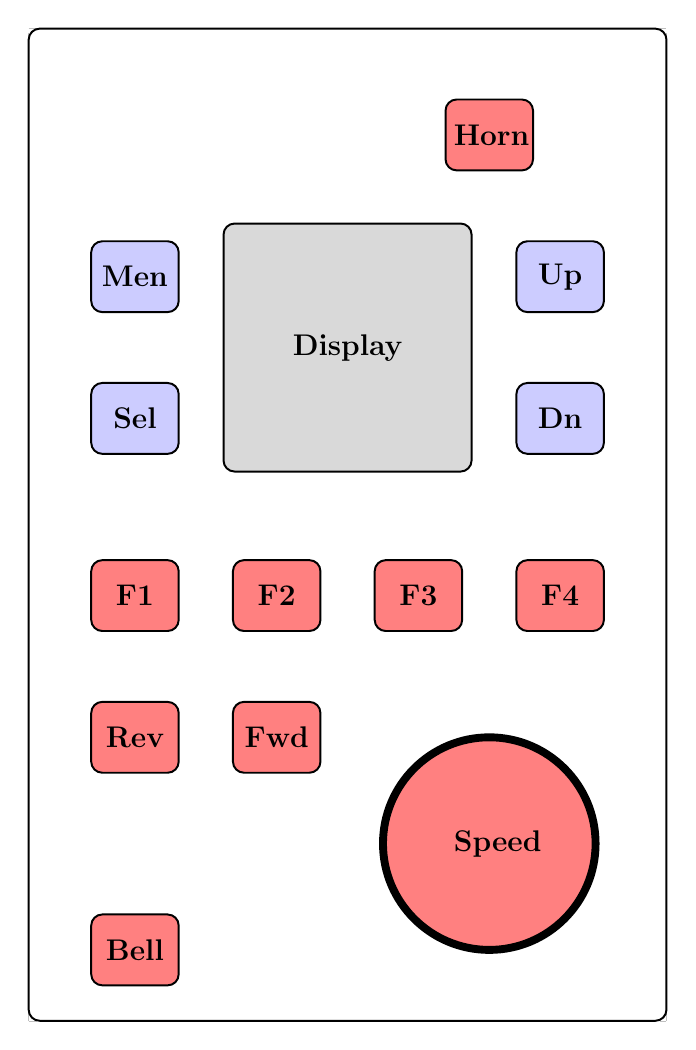
\begin{tikzpicture}[scale=0.9, transform shape]
        
     	\draw[help lines, gray!50, dashed] (0,0) grid(9,14);
     	
     	\node[ tsRoundedRectangle, 
                minimum width=9cm,
                minimum height=14cm,
                text width=3cm,
                text centered,
                fill=white!50] (display) at (4.5,7) {};

       	\node[ tsRoundedRectangle, 
                minimum width=3.5cm,
                minimum height=3.5cm,
                text width=3cm,
                text centered,
                fill=gray!30] (display) at (4.5,9.5) {Display};
        
        \node[ tsRoundedRectangle, 
                minimum width=1cm,
                minimum height=1cm,
                text width=1cm,
                text centered,
                fill=red!50] (horn) at (6.5,12.5) {Horn};
        
        \node[ tsRoundedRectangle, 
                minimum width=1cm,
                minimum height=1cm,
                text width=1cm,
                text centered,
                fill=blue!20] (menu) at (1.5,10.5) {Men};
                
      	\node[ tsRoundedRectangle, 
                minimum width=1cm,
                minimum height=1cm,
                text width=1cm,
                text centered,
                fill=blue!20] (up) at (7.5,10.5) {Up};

     	\node[ tsRoundedRectangle, 
                minimum width=1cm,
                minimum height=1cm,
                text width=1cm,
                text centered,
                fill=blue!20] (sel) at (1.5,8.5) {Sel};
                
    	\node[ tsRoundedRectangle, 
                minimum width=1cm,
                minimum height=1cm,
                text width=1cm,
                text centered,
                fill=blue!20] (down) at (7.5,8.5) {Dn};
                
     	\node[ tsRoundedRectangle, 
                minimum width=1cm,
                minimum height=1cm,
                text width=1cm,
                text centered,
                fill=red!50] (f1) at (1.5,6) {F1};
                
      	\node[ tsRoundedRectangle, 
                minimum width=1cm,
                minimum height=1cm,
                text width=1cm,
                text centered,
                fill=red!50] (f2) at (3.5,6) {F2};
                
      	\node[ tsRoundedRectangle, 
                minimum width=1cm,
                minimum height=1cm,
                text width=1cm,
                text centered,
                fill=red!50] (rev) at (1.5,4) {Rev};
                
      	\node[ tsRoundedRectangle, 
                minimum width=1cm,
                minimum height=1cm,
                text width=1cm,
                text centered,
                fill=red!50] (fwd) at (3.5,4) {Fwd};
                
      	\node[ tsRoundedRectangle, 
                minimum width=1cm,
                minimum height=1cm,
                text width=1cm,
                text centered,
                fill=red!50] (f3) at (5.5,6) {F3};
                
     	\node[ tsRoundedRectangle, 
                minimum width=1cm,
                minimum height=1cm,
                text width=1cm,
                text centered,
                fill=red!50] (f4) at (7.5,6) {F4};
                
       	\node[ tsRoundedRectangle, 
                minimum width=1cm,
                minimum height=1cm,
                text width=1cm,
                text centered,
                fill=red!50] (Bell) at (1.5,1) {Bell};
                
      	\node[ tsCircle,
         		minimum width=3cm,
                minimum height=3cm,
                text width=1cm,
                text centered,
                fill=red!50] (speed) at (6.5,2.5) {Speed};
         
    \end{tikzpicture}
\end{center}

Configuration and part of operation takes place with four buttons, which surround the screen display. The MENU button allows to toggle through the menus defined. To select a menu, the SELECT button is used. The menu toggle and select scheme can be nested. Within a menu screen, the MENU, UP and DOWN buttons are used screen specific and the SELECT button typically confirms the selected action. The direction buttons REV and FWD and the SPEED knob set the speed and direction of the locomotive or consist. F1 to F4 are four general buttons that can be mapped to special functions of the particular locomotive. The Horn and Bell button are rounding up the initial design.

The screen itself has also a common structure for all data displayed. 

// ??? perhaps move into the picture above ?


\begin{center}
    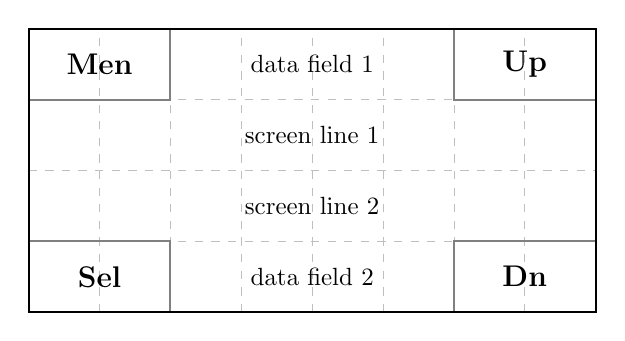
\begin{tikzpicture}[scale=0.9, transform shape]
        
     	\draw[	help lines, gray!50, dashed] (0,0) grid(8,4);
     	
    	       	\node[	tsRectangle, 
     	 		minimum width=2cm,
                minimum height=1cm,
                text width=1cm,
                text centered,
                draw=gray,
                fill=none] (men) at (1,3.5) {Men};
                
      	\node[	tsRectangle, 
     	 		minimum width=2cm,
                minimum height=1cm,
                text width=1cm,
                text centered,
                draw=gray,
                fill=none] (up) at (7,3.5) {Up};
                
       	\node[	tsRectangle, 
     	 		minimum width=2cm,
                minimum height=1cm,
                text width=1cm,
                text centered,
                draw=gray,
                fill=none] (sel) at (1,0.5) {Sel};
                
       	\node[	tsRectangle, 
     	 		minimum width=2cm,
                minimum height=1cm,
                text width=1cm,
                text centered,
                draw=gray,
                fill=none] (down) at (7,0.5) {Dn};
                
        \node[	tsRectangle, 
     	 		minimum width=8cm,
                minimum height=4cm,
                text width=4cm,
                text centered,
                fill=none] (screen) at (4,2) { };
               
		\node at (4,3.5) {data field 1};
		\node at (4,0.5) {data field 2};
		\node at (4,2.5) {screen line 1};
		\node at (4,1.5) {screen line 2};
       
    \end{tikzpicture}
\end{center}

The screen display has several fields. The corner field match the buttons MENU, SEL, UP and DONW. The field width is four characters. The text shown is screen dependent. Typically the action of the four buttons is shown. Between the two corner fields on the top and on the button, there is a data field with up to eight characters. Finally, there are two screen lines in the center of the screen. 

As always, there are many options to build a cab handheld. Although this version connects via cable to the LCS Bus, a wireless version is not hard to build. Having more buttons or fewer buttons, having a set of numeric keypad style input, are all quite valid options. It is a matter of what is preferred. Currently, the cab handheld will not offer any controls for accessories, such as turnouts. This is a subject better left to the layout control panels and controlling software. Our cab handheld favors the approach to model more of a locomotive control stand rather than a TV remote style handheld. Since this is a matter of taste and preference, go build your own.

There is certainly the option to connect commercially available handhelds. This would require to provide a gateway from let's say a LocoNet protocol based handheld to the LCS protocol. Refer to the base station part where it shows an optional LocoNet interface. Well, one day you should be able to connect such handhelds via the LocoNet bus. But right now the topic is on the backlog list.

 	\chapter{The Cab Handheld}

Cab handhelds are used to control a locomotive. Depending on the other capabilities they can also configure a decoder device or set a turnout. Handhelds are connected to the bus, for example LocoNet, sometimes there is a separate bus for just the handhelds. Traditionally a cable connects the handheld to access points on the layout. Just like it is the case for base stations and boosters there is no shortage of cab handhelds. Lately, wireless handhelds have become very popular. And not to forget, some base station integrate handhelds directly in their front panel.

This chapter will describe a general handheld to just control locomotives. It directly connects via cable to the LCS bus and provides the generic elements to specify the locomotive to operate, set the speed and direction as well as the function keys. Implementing a base station and a handheld is all you would need to run an engine and finally see something for your hard work of building a layout system. The cab handheld described first is a board for developing the firmware. Nevertheless it can be used as a full functioning cab handheld. Later version will build upon the firmware but use a more handy form factor.

\section{Requirements}

A cab handheld needs to be able to control the loco. This implies that there is a local non-volatile memory that allows to remember locomotives once controlled. This way one can easily switch between a small set of locomotives and their characteristics. A display will show the actual state of cab handheld and allows together with the configuration buttons to configure the cab handheld. Looking at commercially available handhelds, they all seem to resemble TV controls. A numeric keyboard, some up and down buttons and the speed knob. ( No offense ). In all fairness, they are built to control not only the engines but also the rest of the layout.

But how about a cab handheld that features instead of all the functions to control an entire layout just the features to control an engine. Our cab handheld will have dedicated buttons and levers for let's say a horn or whistle, a bell, and so on. There are also configuration buttons, dedicated buttons and switches, and a very small set of buttons to map to loco specific functions. Furthermore, there is of course the rotary knob for setting the locomotive speed. The following figure shows a rough sketch of the cab handheld elements.

\begin{center}
    \begin{tikzpicture}[scale=0.9, transform shape]
        
     	\draw[help lines, gray!50, dashed] (0,0) grid(9,14);
     	
     	\node[ tsRoundedRectangle, 
                minimum width=9cm,
                minimum height=14cm,
                text width=3cm,
                text centered,
                fill=white!50] (display) at (4.5,7);

       	\node[ tsRoundedRectangle, 
                minimum width=3.5cm,
                minimum height=3.5cm,
                text width=3cm,
                text centered,
                fill=gray!30] (display) at (4.5,9.5) {Display};
        
        \node[ tsRoundedRectangle, 
                minimum width=1cm,
                minimum height=1cm,
                text width=1cm,
                text centered,
                fill=red!50] (horn) at (6.5,12.5) {Horn};
        
        \node[ tsRoundedRectangle, 
                minimum width=1cm,
                minimum height=1cm,
                text width=1cm,
                text centered,
                fill=blue!20] (menu) at (1.5,10.5) {Men};
                
      	\node[ tsRoundedRectangle, 
                minimum width=1cm,
                minimum height=1cm,
                text width=1cm,
                text centered,
                fill=blue!20] (up) at (7.5,10.5) {Up};

     	\node[ tsRoundedRectangle, 
                minimum width=1cm,
                minimum height=1cm,
                text width=1cm,
                text centered,
                fill=blue!20] (sel) at (1.5,8.5) {Sel};
                
    	\node[ tsRoundedRectangle, 
                minimum width=1cm,
                minimum height=1cm,
                text width=1cm,
                text centered,
                fill=blue!20] (down) at (7.5,8.5) {Dn};
                
     	\node[ tsRoundedRectangle, 
                minimum width=1cm,
                minimum height=1cm,
                text width=1cm,
                text centered,
                fill=red!50] (f1) at (1.5,6) {F1};
                
      	\node[ tsRoundedRectangle, 
                minimum width=1cm,
                minimum height=1cm,
                text width=1cm,
                text centered,
                fill=red!50] (f2) at (3.5,6) {F2};
                
      	\node[ tsRoundedRectangle, 
                minimum width=1cm,
                minimum height=1cm,
                text width=1cm,
                text centered,
                fill=red!50] (rev) at (1.5,4) {Rev};
                
      	\node[ tsRoundedRectangle, 
                minimum width=1cm,
                minimum height=1cm,
                text width=1cm,
                text centered,
                fill=red!50] (fwd) at (3.5,4) {Fwd};
                
      	\node[ tsRoundedRectangle, 
                minimum width=1cm,
                minimum height=1cm,
                text width=1cm,
                text centered,
                fill=red!50] (f3) at (5.5,6) {F3};
                
     	\node[ tsRoundedRectangle, 
                minimum width=1cm,
                minimum height=1cm,
                text width=1cm,
                text centered,
                fill=red!50] (f4) at (7.5,6) {F4};
                
       	\node[ tsRoundedRectangle, 
                minimum width=1cm,
                minimum height=1cm,
                text width=1cm,
                text centered,
                fill=red!50] (Bell) at (1.5,1) {Bell};
                
      	\node[ tsCircle,
         		minimum width=3cm,
                minimum height=3cm,
                text width=1cm,
                text centered,
                fill=red!50] (speed) at (6.5,2.5) {Speed};
         
    \end{tikzpicture}
\end{center}

Configuration and part of operation takes place with four buttons, which surround the screen display. The MENU button allows to toggle through the menus defined. To select a menu, the SELECT button is used. The menu toggle and select scheme can be nested. Within a menu screen, the MENU, UP and DOWN buttons are used screen specific and the SELECT button typically confirms the selected action. The direction buttons REV and FWD and the SPEED knob set the speed and direction of the locomotive or consist. F1 to F4 are four general buttons that can be mapped to special functions of the particular locomotive. The Horn and Bell button are rounding up the initial design.

The screen itself has also a common structure for all data displayed. 

\begin{center}
    \begin{tikzpicture}[scale=0.9, transform shape]
        
     	\draw[	help lines, gray!50, dashed] (0,0) grid(8,4);
     	
    	       	\node[	tsRectangle, 
     	 		minimum width=2cm,
                minimum height=1cm,
                text width=1cm,
                text centered,
                draw=gray,
                fill=none] (men) at (1,3.5) {Men};
                
      	\node[	tsRectangle, 
     	 		minimum width=2cm,
                minimum height=1cm,
                text width=1cm,
                text centered,
                draw=gray,
                fill=none] (up) at (7,3.5) {Up};
                
       	\node[	tsRectangle, 
     	 		minimum width=2cm,
                minimum height=1cm,
                text width=1cm,
                text centered,
                draw=gray,
                fill=none] (sel) at (1,0.5) {Sel};
                
       	\node[	tsRectangle, 
     	 		minimum width=2cm,
                minimum height=1cm,
                text width=1cm,
                text centered,
                draw=gray,
                fill=none] (down) at (7,0.5) {Dn};
                
        \node[	tsRectangle, 
     	 		minimum width=8cm,
                minimum height=4cm,
                text width=4cm,
                text centered,
                fill=none] (screen) at (4,2);
               
		\node at (4,3.5) {data field 1};
		\node at (4,0.5) {data field 2};
		\node at (4,2.5) {screen line 1};
		\node at (4,1.5) {screen line 2};
       
    \end{tikzpicture}
\end{center}

The screen display has several fields. The corner field match the buttons MENU, SEL, UP and DONW. The field width is four characters. The text shown is screen dependent. Typically the action of the four buttons is shown. Between the two corner fields on the top and on the button, there is a data field with up to eight characters. Finally, there are two screen lines in the center of the screen. 

\section{Cab Handheld Firmware Development Platform}

A cab handheld as shown in the sketch above consists of the controller portion and a set of buttons and dials. Usually, for the very first steps in firmware design a breadboard implementation of the hardware is used. But why not just create a PCB with all the user elements on it? From experience with breadboards, this setup is by far more robust and you will not chase firmware bugs that turn out to be just a loose connection on a breadboard. This is by the way a lesson learned. With the very reasonable prices for a PCB board, it is almost easier to build a PCB rather early in the design phase and if it has an error, just correct it and order another set of PCBs. Although one could also build the module on a an experimental PCB board, having the schematics done, it is a small step to a dedicated PCB. Definitively worth the small extra effort of making a robust prototype PCB. The following schematic shows the extension board developed for the can handheld firmware development. First, here is the block diagram.

\begin{figure}[ht]
    \centering
    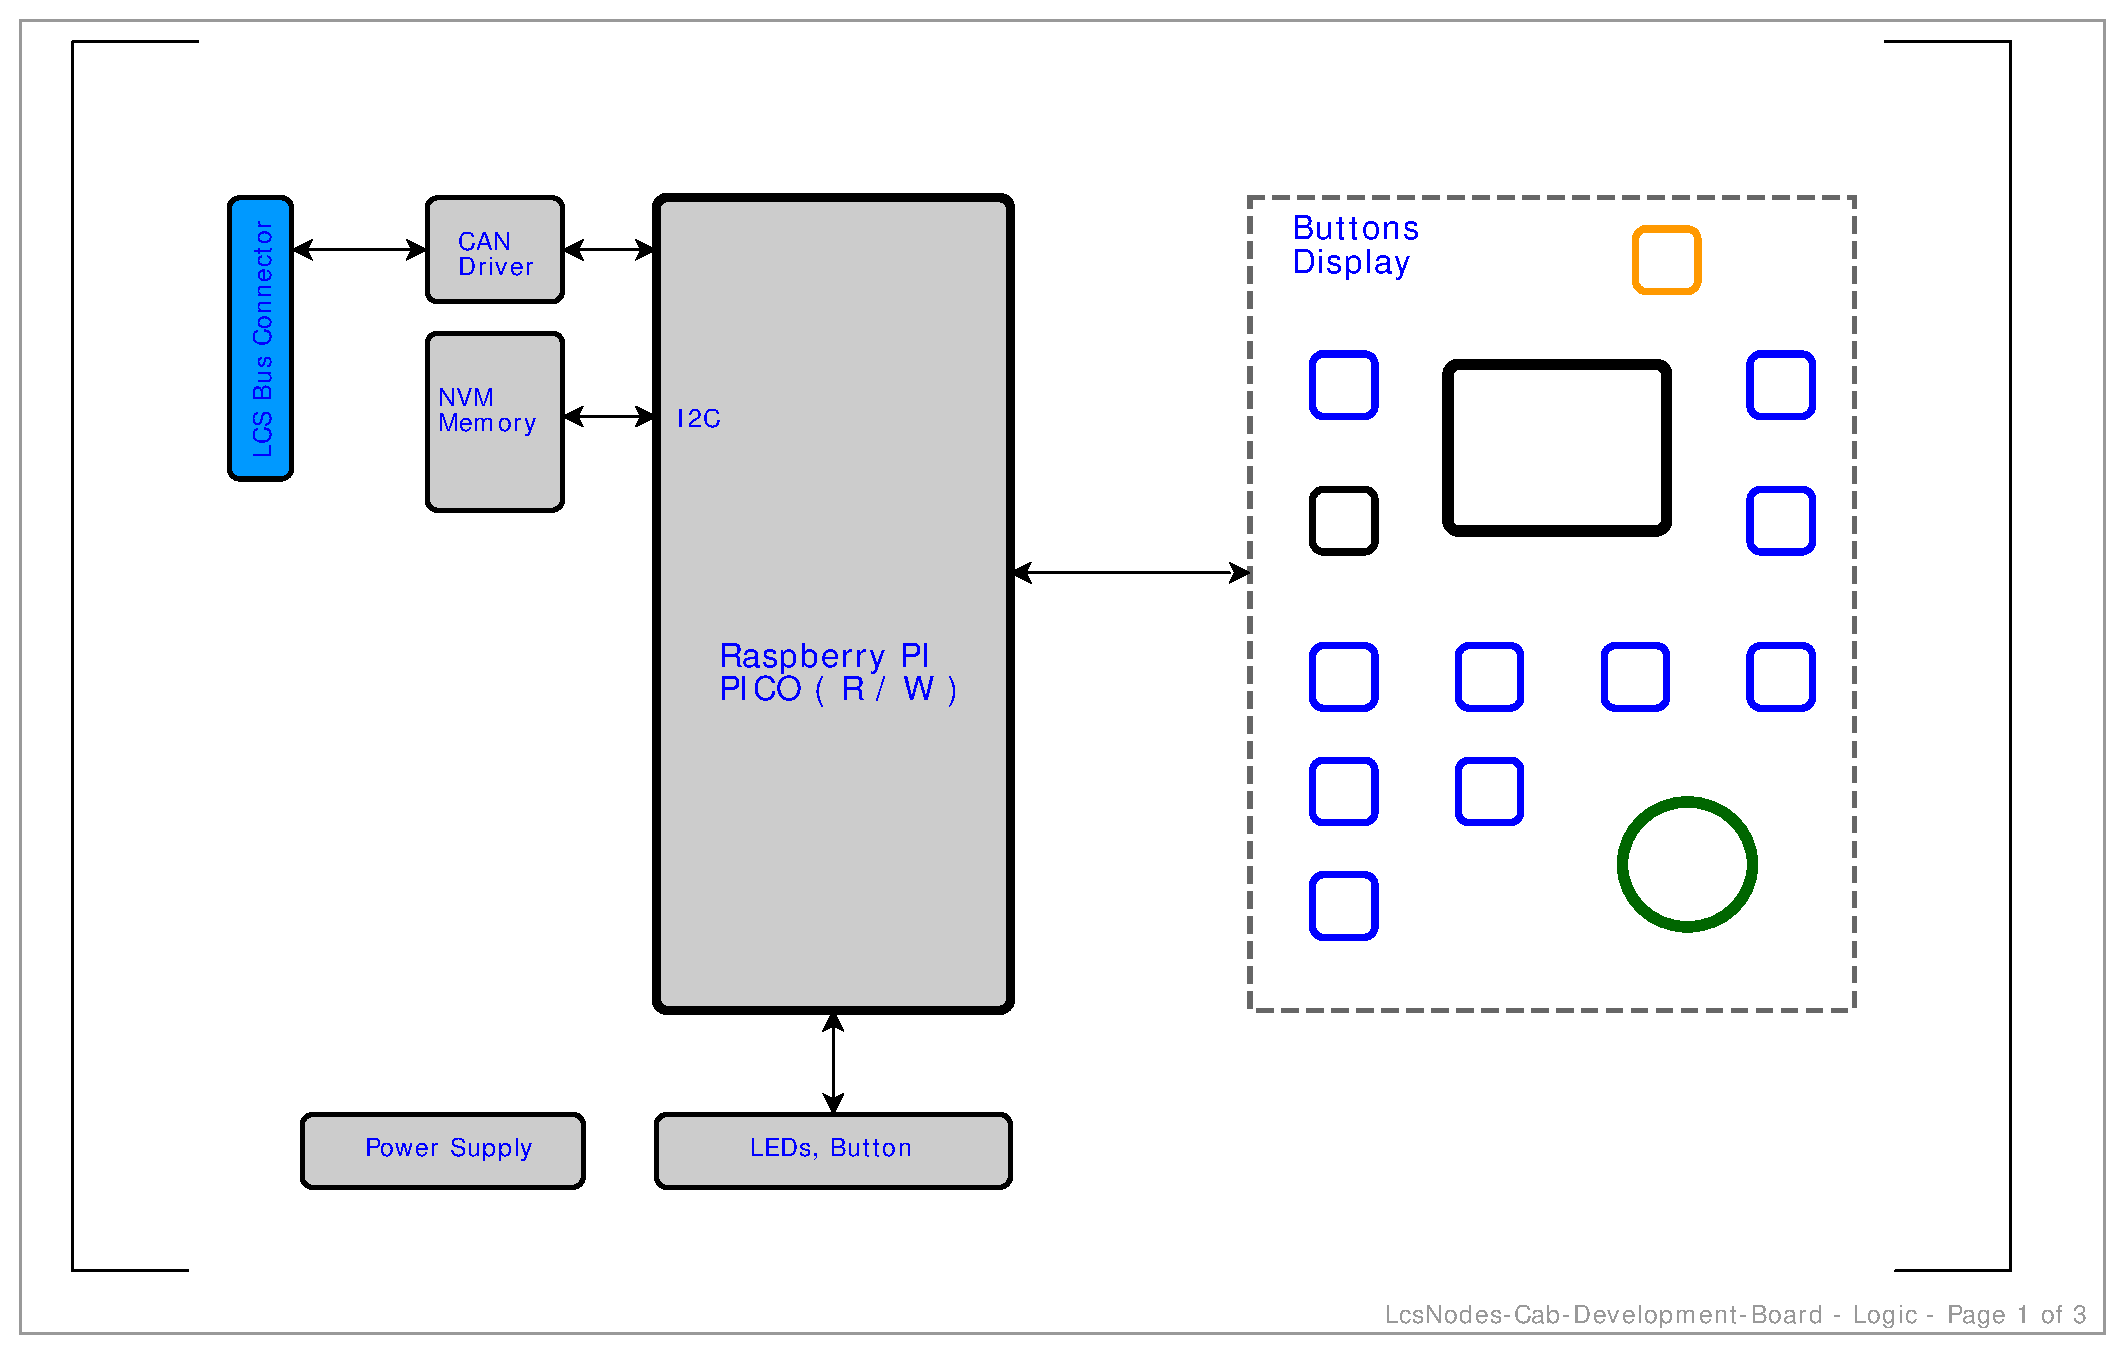
\includegraphics[page=1, width=0.9\textwidth]{./Schematics/Schematic_LcsNodes-Cab-Dev.pdf}
    \caption{Block Diagram}
    %\label{fig:schematic}
\end{figure}

There is essentially a main controller part with the Raspberry Pi Pico, a CAN bus interface and the non-volatile memory. This part should be very familiar by now. Besides the two I2C connections and the CAN bus pins, almost all GPIO pins are dedicated to a button or encoder. Since the GPIOs can be configured with internal pull-up, no external resistors are necessary. The power supply will be fed from the LCS bus. The whole board can also be fed from the USB port of the PICO. Again, this is very handy for initial debugging the firmware. The LCS Bus connector will connect the cab handheld to the LCS layout. We use only the CAN Bus lines and optional the power line input.

\begin{figure}[htbp]
    \centering
    \includegraphics[page=2, width=0.9\textwidth]{./Schematics/Schematic_LcsNodes-Cab-Dev.pdf}
    \caption{Controller}
    %\label{fig:schematic}
\end{figure}
\FloatBarrier

Finally, there is the part with all the buttons, encoders and the OLED Display. The following schematic completes the cap handheld schematic for firmware development.

\begin{figure}[htbp]
    \centering
    \includegraphics[page=3, width=0.9\textwidth]{./Schematics/Schematic_LcsNodes-Cab-Dev.pdf}
    \caption{UI Elements}
    %\label{fig:schematic}
\end{figure}
\FloatBarrier

Granted, it is not really a cab handheld to hold in your hands. Although the final version will have pretty much the same hardware ingredients, the form factor needs to be different. But for development, the setup will be quite helpful and robust. You will avoid chasing software problems that turn out to be just a loose connection on a breadboard. 

\section{A basic Cab Handheld}

As the name already suggests, the cab handheld is a handheld device with several buttons and a display. To keep it a compact design, we will use both sides of the PCB. The upper side contains the buttons, switches and display, the lower side contains the controller components. The cab handheld will connect via a cable to the LCS bus. Power comes from the LCS bus power lines and the CAN bus interface is used to transmit the messages. Perhaps a later version will also add some WLAN capabilities. While WLAN would come pretty much for free with the PICO W, the power supply side needs to include a battery.

\begin{itemize}
\item a 8x12cm board, used from both sides (?)
\item block diagram...
\item power supply from the LCS bus lines
\item controller, a PICO
\item small display
\item rotary encoder, switches, buttons, etc.
\item a subset for analog ?
\end{itemize}

// ??? \textbf{note} to do ..... focus on the firmware first ...

\section{Cab Handheld Firmware}

Now that the development platform is in place, let's have a look at the firmware design. As you perhaps have guessed it, the hardware was already developed with a certain mode in mind. First of all, a cab handheld is nothing else than just another node on the LCS bus. The firmware sits on top of the LCS core library. In addition, there is another key library we have not talked about yet. A cab handheld and also any other device that allows for users to interact, needs software to work with buttons, encoders, displays and so on. This the tasks of the \textbf{UI Elements } library. We will look at this library in a later chapter in great detail.

// ??? note perhaps a picture ?

\begin{itemize}
\item SW architecture on top of the LCS library
\item UI is key to build a handheld
\item firmware to handle the buttons, switches, display, etc. Refer to UIElements.
\item issues LCS messages to the base station for speed, direction and functions
\item menu descriptions
\end{itemize}

\subsection{Concepts}

\begin{itemize}
\item a current cab and a stack of cabs to select from
\item base station has the ultimate data about a cab, loaded into the cab handheld
\item CabHandheld functions and DCC functions
\end{itemize}

\subsection{Screen Layout}

\begin{itemize}
\item display has 4 lines up to 16 characters. Two fonts
\item four navigation buttons, use top and bottom line, 8x8 font
\item two data lines between, 8x16 font.
\end{itemize}

\subsection{Screen Navigation}

\begin{itemize}
\item inherent in the UI Elements Screen Object design
\item MENU
\item SELECT
\item UP
\item DOWN
\end{itemize}

\subsection{Operate Screen}

\begin{itemize}
\item main screen, workhorse
\item speed, dir, functions
\end{itemize}

\subsection{Engine On/off Screen}

\begin{itemize}
\item for diesels only
\end{itemize}

\subsection{Engine Lights Screen}

\begin{itemize}
\item front and back lights...
\end{itemize}

\subsection{New Cab Screen}

There needs to be a way to set an engine cab number. The NEW CAB screen is used to enter a cab Id and engine type. We will display 4 digits and the engine type among we can toggle with the MENU button. The UP/DOWN buttons advance the current digit position. The encoder knob offers a fast way to scroll a digit. The high value digit allows to set an "S" instead of the number to indicate a short loco DCC address. The SELECT button completes the number entering and the current cab becomes this new cab. Note, that it would need to be explicitly saved.

\begin{itemize}
\item works on current cab setting
\end{itemize}

\subsection{Select Cab Screen}

A cab handheld maintains a stack of known cabs. That is cabs the handheld has used before and saved in the cab stack. This menu will toggle through them and select the new current cab. The UP/DOWN button is used to scroll around. In addition, the encoder knob allows to scroll a bit faster. The SELECT button will make the entry shown the current loco.

\begin{itemize}
\item SELECT scrolls through the cab stack and sets the cab selected as current cab.
\end{itemize}

\subsection{Save Cab Screen}

The current cab can be saved in the cab stack. This menu will toggle through them and select the cab slot for saving the current cab data. The UP/DOWN button is used to scroll around. In addition, the encoder knob allows to scroll a bit faster. The SELECT button will perform the action.

\begin{itemize}
\item SAVE scrolls through the cab stack and saves the current cab to this slot.
\item any previous entry used for the same cabId is cleared.
\end{itemize}

\subsection{Set DCC Function}

The DCC standard defines a list of 69 functions, F0 to F68.

\begin{itemize}
\item allows to set any DCC function ( F0 to F68 )
\item encoder knob for fast scrolling
\end{itemize}

\subsection{Config Cab Handheld Functions}

\begin{itemize}
\item connects a cab handheld function to a DCC function
\end{itemize}

\subsection{Options}

\begin{itemize}
\item all kinds of screen for configuration settings
\end{itemize}

\subsection{Diag}

\begin{itemize}
\item all kinds of screen for technical checks and tests
\end{itemize}

\subsection{Summary}

Phew. The cab handheld is another big step toward in operating a layout. After all, a layout control system without some form cab handhelds is not very useful. As said, there are many ways to build a cab. The design of UI elements and firmware was greatly influenced by a handheld called \textbf{\textit{Protothrottle}}. The concept of the four screen menu control buttons found its way into the UI Elements library. In addition to the general cab handheld, a cab handheld tailored toward a specific class of engines would be a great addition to operating that engine. The next section will present a diesel cab handheld that resembles a diesel cab stand from the 1950s.

\section{The Diesel Cab Handheld}

The general handheld for controlling a locomotive is just one possible implementation. There is a company, Iowa Scale Engineering, that has built a handled called the \textbf{\textit{Protothrottle}}. This wireless handheld implements as the control elements the cab of a diesel engine. Wow. There is a lever for the diesel engine prime mover, a level for the direction and one for the brakes. You operate the engine with setting the prime mover notch, release the brakes and then the engine moves. When putting the prime mover to "idle", the engine just roll until you apply the brakes. In short, a much more realistic way to operate a diesel locomotive. 

The diesel cab handheld will leverage many of the design elements of the general cab handheld. There is a display surrounded by the four buttons MENU, SEL, UP and DOWN. The software configuration menus follow the same principles. There are the four function buttons, the horn and the bell. Where the layout differs is that there is no knob for the speed. Instead throttle and brake levers are available. Also, the direction is modeled as a lever instead of two buttons. The following figure shows a rough sketch of the diesel cab handheld.

\begin{center}
    \begin{tikzpicture}[scale=0.9, transform shape]
        
     	\draw[help lines, gray!50, dashed] (0,0) grid(9,14);
     	
     	\node[ tsRoundedRectangle, 
                minimum width=9cm,
                minimum height=14cm,
                text width=3cm,
                text centered,
                fill=white!50] (display) at (4.5,7);

       	\node[ tsRoundedRectangle, 
                minimum width=3.5cm,
                minimum height=3.5cm,
                text width=3cm,
                text centered,
                fill=gray!30] (display) at (4.5,9.5) {Display};
        
        \node[ tsRoundedRectangle, 
                minimum width=1cm,
                minimum height=1cm,
                text width=1cm,
                text centered,
                fill=red!50] (horn) at (6.5,12.5) {Horn};
        
        \node[ tsRoundedRectangle, 
                minimum width=1cm,
                minimum height=1cm,
                text width=1cm,
                text centered,
                fill=blue!20] (menu) at (1.5,10.5) {Men};
                
      	\node[ tsRoundedRectangle, 
                minimum width=1cm,
                minimum height=1cm,
                text width=1cm,
                text centered,
                fill=blue!20] (up) at (7.5,10.5) {Up};

     	\node[ tsRoundedRectangle, 
                minimum width=1cm,
                minimum height=1cm,
                text width=1cm,
                text centered,
                fill=blue!20] (sel) at (1.5,8.5) {Sel};
                
    	\node[ tsRoundedRectangle, 
                minimum width=1cm,
                minimum height=1cm,
                text width=1cm,
                text centered,
                fill=blue!20] (down) at (7.5,8.5) {Dn};
                
     	\node[ tsRoundedRectangle, 
                minimum width=1cm,
                minimum height=1cm,
                text width=1cm,
                text centered,
                fill=red!50] (f1) at (1.5,6) {F1};
                
      	\node[ tsRoundedRectangle, 
                minimum width=1cm,
                minimum height=1cm,
                text width=1cm,
                text centered,
                fill=red!50] (f2) at (3.5,6) {F2};
                
      	\node[ tsRoundedRectangle, 
                minimum width=1cm,
                minimum height=1cm,
                text width=1cm,
                text centered,
                fill=red!50] (f3) at (5.5,6) {F3};
                
     	\node[ tsRoundedRectangle, 
                minimum width=1cm,
                minimum height=1cm,
                text width=1cm,
                text centered,
                fill=red!50] (f4) at (7.5,6) {F4};
                
      	\node[ tsRoundedRectangle, 
                minimum width=6cm,
                minimum height=0.75cm,
                text width=1cm,
                text centered,
                fill=red!50] (throttle) at (5,4.5) {Throttle};
                
                
       	\node[ tsRoundedRectangle, 
                minimum width=2cm,
                minimum height=0.75cm,
                text width=1cm,
                text centered,
                fill=red!50] (dir) at (6,3) {Dir};
                
      	\node[ tsRoundedRectangle, 
                minimum width=3cm,
                minimum height=0.75cm,
                text width=1cm,
                text centered,
                fill=red!50] (brake) at (2.5,2.5) {Brake};
                
                
       	\node[ tsRoundedRectangle, 
                minimum width=1cm,
                minimum height=1cm,
                text width=1cm,
                text centered,
                fill=red!50] (Bell) at (1.5,1) {Bell};
                
    \end{tikzpicture}
\end{center}


Leveraging the cab handheld hardware from the previous chapter, the diesel cab handheld just differs in the levers for throttle, direction and brake instead of the speed knob. All else is fairly the same. Let's get started.

\subsection{Requirements}

\begin{itemize}
\item Very similar to the previous cab handheld 
\item instead of speed knob, it features throttle and brake.
\item all else is about the same...
\end{itemize}

\subsection{Module hardware}

\begin{itemize}
\item Leverage the generic cab handheld
\item Controller with CanBus interface
\item power supply from the LCS bus lines
\item small display
\item rotary encoder, buttons, etc.
\end{itemize}

\subsection{Module firmware}

\begin{itemize}
\item UI elements are key again, leverage many screen built before
\item new part is how throttle and brake interplay to run the engine
\end{itemize}


\section{Summary}

\begin{itemize}
\item now we have a generic cab handheld and a diesel cab handheld.
\item one could come up with a steam or electric engine handheld. 
\item the firmware already goes a long way to quickly realize further cab handhelds.
\item would we ever build a handheld with other non-engine functionality... who knows... not right now.
\item would we build a version that can be integrated into a |\"Stellwerk\" table ? perhaps... just a main controller and an cab UI Elements extension
\end{itemize}

As always, there are many options to build a cab handheld. Although this version connects via cable to the LCS Bus, a wireless version is not hard to build. Having more buttons or fewer buttons, having a set of numeric keypad style input, are all quite valid options. It is a matter of what is preferred. Currently, the cab handheld will not offer any controls for accessories, such as turnouts. This is a subject better left to the layout control panels and controlling software. Our cab handheld favors the approach to model more of a locomotive control stand rather than a TV remote style handheld. Since this is a matter of taste and preference, go build your own.

There is certainly the option to connect commercially available handhelds. This would require to provide a gateway from let's say a LocoNet protocol based handheld to the LCS protocol. Refer to the base station part where is shows an optional LocoNet interface. Well, one day you should be able to connect such handhelds via the LocoNet bus. But right now the topic is on the backlog list.
 	\chapter{Cab Handheld Firmware}


This chapter will describe the firmware for our cab handhelds. 


 It directly connects via cable to the LCS bus and provides the generic elements to specify the locomotive to operate, set the speed and direction as well as the function keys. Implementing a base station and a handheld is all you would need to run an engine and finally see something for your hard work of building a layout system. The cab handheld described first is a board for developing the firmware. Nevertheless it can be used as a full functioning cab handheld. Later version will build upon the firmware but use a more handy form factor.

\section{Requirements}

A cab handheld needs to be able to control the loco. This implies that there is a local non-volatile memory that allows to remember locomotives once controlled. This way one can easily switch between a small set of locomotives and their characteristics. A display will show the actual state of cab handheld and allows together with the configuration buttons to configure the cab handheld. Looking at commercially available handhelds, they all seem to resemble TV controls. A numeric keyboard, some up and down buttons and the speed knob. ( No offense ). In all fairness, they are built to control not only the engines but also the rest of the layout.

But how about a cab handheld that features instead of all the functions to control an entire layout just the features to control an engine. Our cab handheld will have dedicated buttons and levers for let's say a horn or whistle, a bell, and so on. There are also configuration buttons, dedicated buttons and switches, and a very small set of buttons to map to loco specific functions. Furthermore, there is of course the rotary knob for setting the locomotive speed. The following figure shows a rough sketch of the cab handheld elements.

\begin{center}
    \begin{tikzpicture}[scale=0.9, transform shape]
        
     	\draw[help lines, gray!50, dashed] (0,0) grid(9,14);
     	
     	\node[ tsRoundedRectangle, 
                minimum width=9cm,
                minimum height=14cm,
                text width=3cm,
                text centered,
                fill=white!50] (display) at (4.5,7);

       	\node[ tsRoundedRectangle, 
                minimum width=3.5cm,
                minimum height=3.5cm,
                text width=3cm,
                text centered,
                fill=gray!30] (display) at (4.5,9.5) {Display};
        
        \node[ tsRoundedRectangle, 
                minimum width=1cm,
                minimum height=1cm,
                text width=1cm,
                text centered,
                fill=red!50] (horn) at (6.5,12.5) {Horn};
        
        \node[ tsRoundedRectangle, 
                minimum width=1cm,
                minimum height=1cm,
                text width=1cm,
                text centered,
                fill=blue!20] (menu) at (1.5,10.5) {Men};
                
      	\node[ tsRoundedRectangle, 
                minimum width=1cm,
                minimum height=1cm,
                text width=1cm,
                text centered,
                fill=blue!20] (up) at (7.5,10.5) {Up};

     	\node[ tsRoundedRectangle, 
                minimum width=1cm,
                minimum height=1cm,
                text width=1cm,
                text centered,
                fill=blue!20] (sel) at (1.5,8.5) {Sel};
                
    	\node[ tsRoundedRectangle, 
                minimum width=1cm,
                minimum height=1cm,
                text width=1cm,
                text centered,
                fill=blue!20] (down) at (7.5,8.5) {Dn};
                
     	\node[ tsRoundedRectangle, 
                minimum width=1cm,
                minimum height=1cm,
                text width=1cm,
                text centered,
                fill=red!50] (f1) at (1.5,6) {F1};
                
      	\node[ tsRoundedRectangle, 
                minimum width=1cm,
                minimum height=1cm,
                text width=1cm,
                text centered,
                fill=red!50] (f2) at (3.5,6) {F2};
                
      	\node[ tsRoundedRectangle, 
                minimum width=1cm,
                minimum height=1cm,
                text width=1cm,
                text centered,
                fill=red!50] (rev) at (1.5,4) {Rev};
                
      	\node[ tsRoundedRectangle, 
                minimum width=1cm,
                minimum height=1cm,
                text width=1cm,
                text centered,
                fill=red!50] (fwd) at (3.5,4) {Fwd};
                
      	\node[ tsRoundedRectangle, 
                minimum width=1cm,
                minimum height=1cm,
                text width=1cm,
                text centered,
                fill=red!50] (f3) at (5.5,6) {F3};
                
     	\node[ tsRoundedRectangle, 
                minimum width=1cm,
                minimum height=1cm,
                text width=1cm,
                text centered,
                fill=red!50] (f4) at (7.5,6) {F4};
                
       	\node[ tsRoundedRectangle, 
                minimum width=1cm,
                minimum height=1cm,
                text width=1cm,
                text centered,
                fill=red!50] (Bell) at (1.5,1) {Bell};
                
      	\node[ tsCircle,
         		minimum width=3cm,
                minimum height=3cm,
                text width=1cm,
                text centered,
                fill=red!50] (speed) at (6.5,2.5) {Speed};
         
    \end{tikzpicture}
\end{center}

Configuration and part of operation takes place with four buttons, which surround the screen display. The MENU button allows to toggle through the menus defined. To select a menu, the SELECT button is used. The menu toggle and select scheme can be nested. Within a menu screen, the MENU, UP and DOWN buttons are used screen specific and the SELECT button typically confirms the selected action. The direction buttons REV and FWD and the SPEED knob set the speed and direction of the locomotive or consist. F1 to F4 are four general buttons that can be mapped to special functions of the particular locomotive. The Horn and Bell button are rounding up the initial design.

The screen itself has also a common structure for all data displayed. 

\begin{center}
    \begin{tikzpicture}[scale=0.9, transform shape]
        
     	\draw[	help lines, gray!50, dashed] (0,0) grid(8,4);
     	
    	       	\node[	tsRectangle, 
     	 		minimum width=2cm,
                minimum height=1cm,
                text width=1cm,
                text centered,
                draw=gray,
                fill=none] (men) at (1,3.5) {Men};
                
      	\node[	tsRectangle, 
     	 		minimum width=2cm,
                minimum height=1cm,
                text width=1cm,
                text centered,
                draw=gray,
                fill=none] (up) at (7,3.5) {Up};
                
       	\node[	tsRectangle, 
     	 		minimum width=2cm,
                minimum height=1cm,
                text width=1cm,
                text centered,
                draw=gray,
                fill=none] (sel) at (1,0.5) {Sel};
                
       	\node[	tsRectangle, 
     	 		minimum width=2cm,
                minimum height=1cm,
                text width=1cm,
                text centered,
                draw=gray,
                fill=none] (down) at (7,0.5) {Dn};
                
        \node[	tsRectangle, 
     	 		minimum width=8cm,
                minimum height=4cm,
                text width=4cm,
                text centered,
                fill=none] (screen) at (4,2);
               
		\node at (4,3.5) {data field 1};
		\node at (4,0.5) {data field 2};
		\node at (4,2.5) {screen line 1};
		\node at (4,1.5) {screen line 2};
       
    \end{tikzpicture}
\end{center}

The screen display has several fields. The corner field match the buttons MENU, SEL, UP and DONW. The field width is four characters. The text shown is screen dependent. Typically the action of the four buttons is shown. Between the two corner fields on the top and on the button, there is a data field with up to eight characters. Finally, there are two screen lines in the center of the screen. 


\section{Cab Handheld Firmware}

Now that the development platform is in place, let's have a look at the firmware design. As you perhaps have guessed it, the hardware was already developed with a certain mode in mind. First of all, a cab handheld is nothing else than just another node on the LCS bus. The firmware sits on top of the LCS core library. In addition, there is another key library we have not talked about yet. A cab handheld and also any other device that allows for users to interact, needs software to work with buttons, encoders, displays and so on. This the tasks of the \textbf{UI Elements } library. We will look at this library in a later chapter in great detail.

// ??? note perhaps a picture ?

\begin{itemize}
\item SW architecture on top of the LCS library
\item UI is key to build a handheld
\item firmware to handle the buttons, switches, display, etc. Refer to UIElements.
\item issues LCS messages to the base station for speed, direction and functions
\item menu descriptions
\end{itemize}

\subsection{Concepts}

\begin{itemize}
\item a current cab and a stack of cabs to select from
\item base station has the ultimate data about a cab, loaded into the cab handheld
\item CabHandheld functions and DCC functions
\end{itemize}

\subsection{Screen Layout}

\begin{itemize}
\item display has 4 lines up to 16 characters. Two fonts
\item four navigation buttons, use top and bottom line, 8x8 font
\item two data lines between, 8x16 font.
\end{itemize}

\subsection{Screen Navigation}

\begin{itemize}
\item inherent in the UI Elements Screen Object design
\item MENU
\item SELECT
\item UP
\item DOWN
\end{itemize}

\subsection{Operate Screen}

\begin{itemize}
\item main screen, workhorse
\item speed, dir, functions
\end{itemize}

\subsection{Engine On/off Screen}

\begin{itemize}
\item for diesels only
\end{itemize}

\subsection{Engine Lights Screen}

\begin{itemize}
\item front and back lights...
\end{itemize}

\subsection{New Cab Screen}

There needs to be a way to set an engine cab number. The NEW CAB screen is used to enter a cab Id and engine type. We will display 4 digits and the engine type among we can toggle with the MENU button. The UP/DOWN buttons advance the current digit position. The encoder knob offers a fast way to scroll a digit. The high value digit allows to set an "S" instead of the number to indicate a short loco DCC address. The SELECT button completes the number entering and the current cab becomes this new cab. Note, that it would need to be explicitly saved.

\begin{itemize}
\item works on current cab setting
\end{itemize}

\subsection{Select Cab Screen}

A cab handheld maintains a stack of known cabs. That is cabs the handheld has used before and saved in the cab stack. This menu will toggle through them and select the new current cab. The UP/DOWN button is used to scroll around. In addition, the encoder knob allows to scroll a bit faster. The SELECT button will make the entry shown the current loco.

\begin{itemize}
\item SELECT scrolls through the cab stack and sets the cab selected as current cab.
\end{itemize}

\subsection{Save Cab Screen}

The current cab can be saved in the cab stack. This menu will toggle through them and select the cab slot for saving the current cab data. The UP/DOWN button is used to scroll around. In addition, the encoder knob allows to scroll a bit faster. The SELECT button will perform the action.

\begin{itemize}
\item SAVE scrolls through the cab stack and saves the current cab to this slot.
\item any previous entry used for the same cabId is cleared.
\end{itemize}

\subsection{Set DCC Function}

The DCC standard defines a list of 69 functions, F0 to F68.

\begin{itemize}
\item allows to set any DCC function ( F0 to F68 )
\item encoder knob for fast scrolling
\end{itemize}

\subsection{Config Cab Handheld Functions}

\begin{itemize}
\item connects a cab handheld function to a DCC function
\end{itemize}

\subsection{Options}

\begin{itemize}
\item all kinds of screen for configuration settings
\end{itemize}

\subsection{Diag}

\begin{itemize}
\item all kinds of screen for technical checks and tests
\end{itemize}

\subsection{Summary}

Phew. The cab handheld is another big step toward in operating a layout. After all, a layout control system without some form cab handhelds is not very useful. As said, there are many ways to build a cab. The design of UI elements and firmware was greatly influenced by a handheld called \textbf{\textit{Protothrottle}}. The concept of the four screen menu control buttons found its way into the UI Elements library. In addition to the general cab handheld, a cab handheld tailored toward a specific class of engines would be a great addition to operating that engine. The next section will present a diesel cab handheld that resembles a diesel cab stand from the 1950s.


\section{Summary}

\begin{itemize}
\item now we have a generic cab handheld and a diesel cab handheld.
\item one could come up with a steam or electric engine handheld. 
\item the firmware already goes a long way to quickly realize further cab handhelds.
\item would we ever build a handheld with other non-engine functionality... who knows... not right now.
\item would we build a version that can be integrated into a |\"Stellwerk\" table ? perhaps... just a main controller and an cab UI Elements extension
\end{itemize}

As always, there are many options to build a cab handheld. Although this version connects via cable to the LCS Bus, a wireless version is not hard to build. Having more buttons or fewer buttons, having a set of numeric keypad style input, are all quite valid options. It is a matter of what is preferred. Currently, the cab handheld will not offer any controls for accessories, such as turnouts. This is a subject better left to the layout control panels and controlling software. Our cab handheld favors the approach to model more of a locomotive control stand rather than a TV remote style handheld. Since this is a matter of taste and preference, go build your own.

There is certainly the option to connect commercially available handhelds. This would require to provide a gateway from let's say a LocoNet protocol based handheld to the LCS protocol. Refer to the base station part where is shows an optional LocoNet interface. Well, one day you should be able to connect such handhelds via the LocoNet bus. But right now the topic is on the backlog list.

	\include{chapters/chapter-lcs-block-controller-introduction}
	\include{chapters/chapter-lcs-concepts-signaling-block-control}
 	\include{chapters/chapter-lcs-block-controller-hardware}
 	\include{chapters/chapter-lcs-block-controller-firmware}
 	
 	\chapter{LCS Module - Gateways}

The layout system rests on the CAN Bus and all nodes connect to the bus. But this is only one way to built the foundation. The requirements to connect a computer can be handled via the USB bus of the base station. But also, as the protocol is not bound to the CAN Bus, there is an option to have a gateway to connect other devices via for example an Ethernet protocol. But right now, this is work on the to do list.

\section{Base Station ASCII Interface}

a kind of gateway

\section{LCS Bus Gateway}

issue LCS messages directly from a computer, etc.

\section{LAN Gateway}

issue LCS messages received via LAN, WLAN

\section{LocoNet Gateway}

protocol gateway

translate LocNet messages into LCS messags

\section{Summary}


 	
 
  	%----------------------------------------------------------------------------
 	\part{LCS Extensions}
 	
 	\chapter{Hardware Extension Module Design}

LCS hardware modules typically consist of a controller portion and an extension portion. Welcome to the extension part of hardware module design. To recap, controller boards features an extension connector that contains signal lines to the extension board. This connector provides among other lines an I2C bus, which is the communication bus to elements on the extension boards.

Each hardware module almost certainly has additional requirements. Depending on the module type there will be a great variety of extensions. A good example is the sensor and actor hardware for managing the respective turnouts, signals, and so on. A solution to these family of modules is to use the I2C communication bus and a few more controller lines between controller main board and extensions. Rather than exporting as many as possible pins of the controller via an extension connector, the extension connector presented is hopefully a reasonable compromise when it comes to numbers of pins and capabilities. For complex extension boards with many controller interaction points, a monolithic approach, i.e. controller and extension functionality on one board, would perhaps be the better choice. Such boards could still export the basic functions such as I2C via the extension connector to less complex extension boards for providing additional capabilities. Before we discuss any particular extension board, this chapter will present the hardware and firmware foundation for addressing an extension board.

\section{Requirements}

As with any LCS library part presented, the key goal is to unify and simplify access to an extension board, while still allowing for great flexibility in actual extension board design. We want to be able to connect pretty much any extension board to a main controller, base station and block controller, as well as connecting several extension boards. For example, take the block controller. As shown before, the block controller exports the track power lines and the extension connector. We would like to be able to connect an extension board that implements the track occupancy detectors. We would also like to connect a further extension board that implements the turnout and signal drivers. And of course we want to connect boards then combine one or many of these functions. A key requirement is therefore to communicate to the main controller what is actually connected and how to access the available functions.

\begin{figure}[htbp]
    \centering
    \begin{tikzpicture}[scale=1, transform shape]
        \useasboundingbox (0,0) rectangle (15,6);
        \draw[help lines, gray!50, dashed] (0,0) grid(15,6);

        \node at (3.5, 2.5) {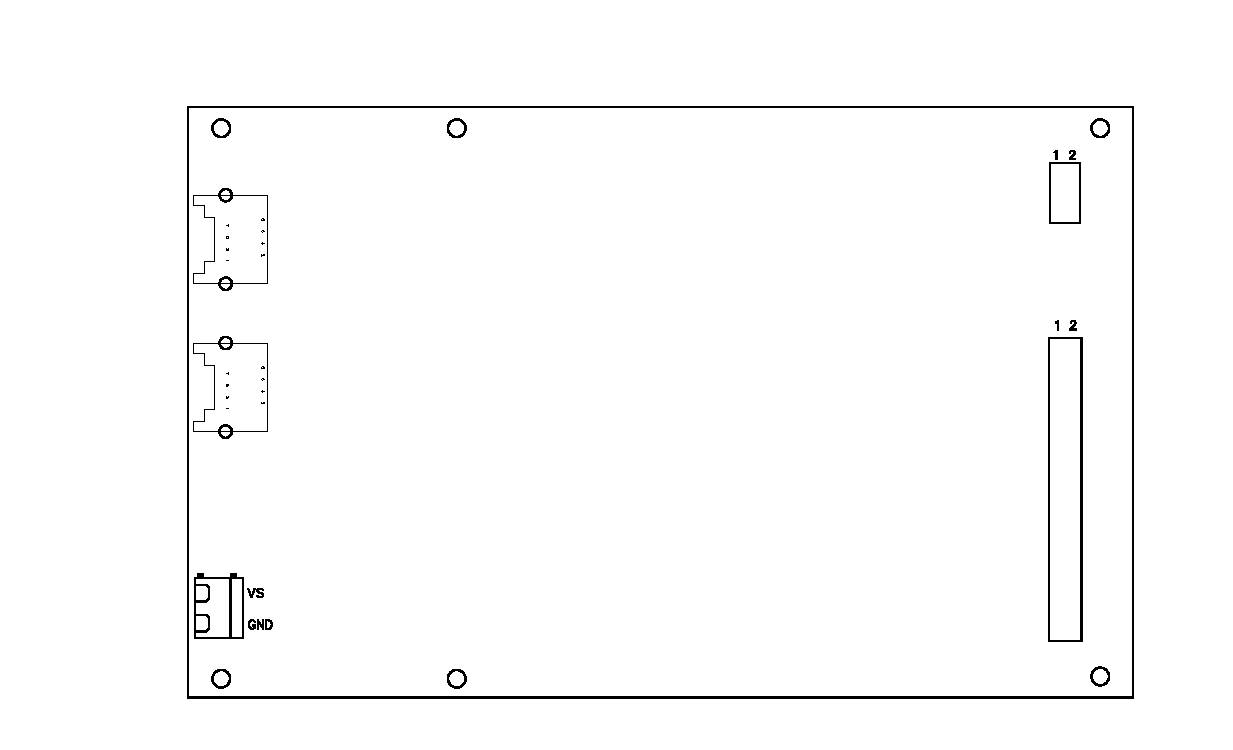
\includegraphics[page=1, width=0.4\textwidth]{./figures/LCS-FP-MAIN-CTRL-Sketch.pdf}};

        \node at (11.5, 2.5) {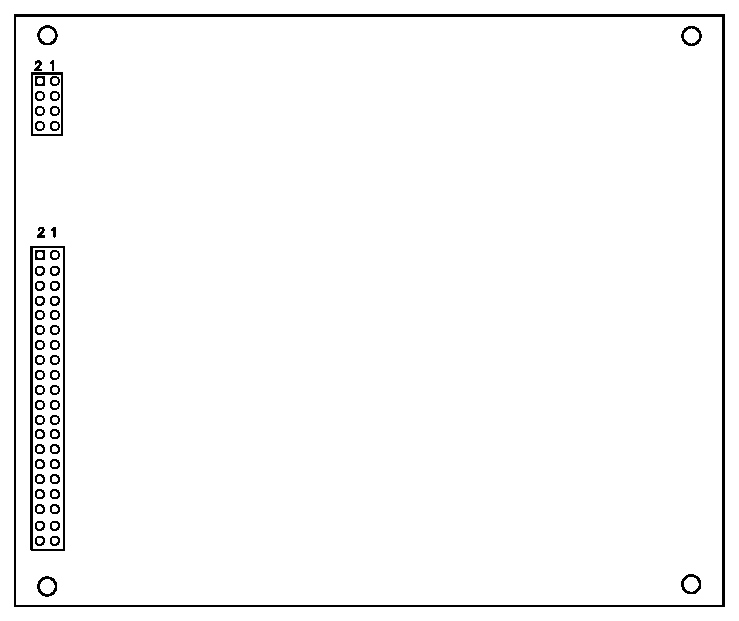
\includegraphics[page=1, width=0.4\textwidth]{./figures/LCS-FP-EXT-L-Sketch.pdf}};

        \node at (3, 5.5) {\textbf{Main Controller}};
        \node at (11, 5.5) {\textbf{Extension Board}};
        \node at (3.5, 4.3) {Track Bus};
        \node at (3.5, 1.7) {Extension Bus};

        \draw[line width=1mm, gray!40, ->] (5, 4.3) -- (11,4.3);
        \draw[line width=1mm, gray!40, ->] (5,1.7) -- (11,1.7);
    
    \end{tikzpicture}
    \caption{Connecting boards}
    %\label{fig:composite-image}
\end{figure}

Typical electronic modules found for digital model railroad control offers configuration options via software and perhaps a set of DIP switches or on board jumpers. As extension boards become more rich in the features they offers and also the combination of more than one board, a methods is needed to uniquely identify and address a board on the extension connectors and a methods to interrogate the capabilities of that particular board.

We already talked about the ability to connect more than one extension board. When this is the case, the order of connected boards should not matter as long as they are uniquely identified. A method is needed for the main controller to automatically identify all extension boards at startup along with their capabilities, ie.e the functions they offer. Other than the methods describing what the board can actually do, the extension board will not have any non-volatile state.

Because of the large variety of extension boards a software layer is needed that unifies how the individual access points such as a digital input or output is accessed by the LCS node firmware. There should be an easy and uniform way to address these endpoints, i.e. there should be some kind of an \textbf{extension library} interface common to all extension boards designed.

The upper layer, i.e. the extension library interface, is complemented by the lower layer which is actually the piece of code that know the extension hardware and translates a higher lever library call into the sequence of actions on the particular extension board. This piece of code will be called \textbf{extension driver}. For each extension board or family of alike boards there is at least one such driver.

\section{Concepts}

To accommodate the requirements, each extension board has to a hardware mechanism that uniquely identifies the board and its capabilities. It is a not a requirement that such a board has processing power or retains any state. This is the responsibility of the controller board. When power is applied to the main controller the reset or restart sequence will attempt to discover all extension boards connected. For this to work, each board has a non-volatile memory structure that describes the board capabilities. And this memory needs to be at a known place, i.e. I2C address, such that this information can be read without knowing any further details. For this purpose, extension boards will have a NVM chip, that contains the board description.

The NVM chip is "programmed" by writing the relevant data to the chip. A write-enable jumper is used to allow writing and then disable all further changes during operation. There is no need for a special programmer, any main controller board can do this via the I2C lines of the extension connector. With using the NV chip, there is no need to have any further DIP switches or alike on the board. In fact, a memory chip allows for even more precise options to configure. And it is cheaper that even a 4-DIP switch.

After programming the NVM chip will contains all information needed to address the extension board functions. Typically, one or more I2C addressable chips are on the board and the NVM tells us what their address is. Combining the chip foxed I2C address portion, the board address portion and the individual chip select portion, an I2C bus unique address is formed. 

The software library can now access a chip. However, chips vary greatly in their functions and how they are controlled by software. A concept is needed to communicate with these chops at  higher abstraction level. Think of a driver in operating systems. A driver offers a set of routines, such as open, read, write and close and takes care of the underlying details how to talk to the physical object. We will go a similar route. There is a high level library, the extension library that offers a high level view of extension board capabilities. Upon node reset and restart, the controller board will query the NVM chips on the extension bod and dynamically configure the driver code for this board.

In addition to the board address a large variety of inputs, outputs and perhaps functions need to be address too. We will call them endpoints. Consider  16-port digital IO chip, such as the MCP23017. It will have 16 IO pins, which we call 16 endpoints. Uniquely identifying an and point is to know the board ID and the endpoint Id on that board. Again, all this information is stored in the NVM  chip at extension board conjuration time. An endpoint could be a variety of things. For example a plan digital output, a servo output, and analog input, and so on. An endpoint could also be a logical entity that groups multiple pins or issue a series of commands to the extension board.

For a new board design, the development process is therefore to define the NVM data that represent the hardware capabilities  and to provide a driver for the board capabilities. From thereon, the firmware designer can use the extension boards with simple but powerful commands. How does this all map to LCS nodes and ports ? Well, the firmware designer has to provide the code that makes the respective driver calls when receiving node and port control commands and events.

\section{I2C Addressing}

An extension board design assumes that the key ICs on the board are I2C addressable chips. As already mentioned, I2C ICs have a fixed I2C address part and a some address bits that can be set by hardware. Most of the I2C chips used in our designs have a four bit fixed address portion and a configurable portion to be supplied via address pins of the chip. We will use the configurable portion to identify the board, from A2 to A1 and reserve the last bit A0 for selecting two chips of the same kind on an extension board.


\begin{longtable}{@{}|l|l|l|l|l|l|l|l|p{0.3\linewidth}|@{}}
    \caption{I2C Chip} \\
    \toprule
    \textbf{IC} & \textbf{A6} & \textbf{A5} & \textbf{A4} & \textbf{A3} & \textbf{A2} & \textbf{A1} & \textbf{A0} & \textbf{Type} \\
    \midrule
    \endfirsthead
    \toprule
    \textbf{IC} & \textbf{A6} & \textbf{A5} & \textbf{A4} & \textbf{A3} & \textbf{A2} & \textbf{A1} & \textbf{A0} & \textbf{Type} \\
    \midrule
    \endhead
    \midrule
    \multicolumn{5}{r}{\textit{Continued on next page}} \\
    \midrule
    \endfoot
    \bottomrule
    \endlastfoot
    \textbf{MCP23017} & 0 & 1 & 0 & 0 & B1 & B0 & x & 16 port DIO \\
    \midrule
    \textbf{PCA9555} & 0 & 1 & 0 & 0 & B1 & B0 & x & 16 port DIO \\
    \midrule
    \textbf{PCA9955} & 1 & 1 & 0 & 1 & B1 & B0 & x & 16 port LED driver \\
    \midrule
    \textbf{PCA9685} & 1 & 1 & 1 & 1 & B1 & B0 & x & 16 port servo driver \\
    \midrule
    \textbf{24AA128} & 1 & 0 & 1 & 0 & B1 & B0 & x & Non volatile memory \\
    \midrule
    \textbf{24AA256} & 1 & 0 & 1 & 0 & B1 & B0 & x & Non volatile memory \\
    \midrule
    \textbf{24AA512} & 1 & 0 & 1 & 0 & B1 & B0 & x & Non volatile memory \\
\end{longtable}%

The PCA 9955 and 9685 have a high number of address selection inputs. This allows to connect more than typically 8 chips on one I2C bus. We will not make use of this capability for now and assign a fixed 4-bit chip I2C address portion.

\section{Multiple Extension Boards}

Now that we talked about I2C address, how does a board get a unique board address without jumpers or alike ? Each board must have a way to contribute to an I2C address its own portion. When an I2C address is sent on the bus, it will have a board ID, this ID is used in the final I2C address. Each extension board features a common set of circuitry for this purpose. The following schematic shows the connectors, the board address generation logic and the NMV chip.

\begin{tikzpicture}[scale=0.9, transform shape]

    \draw[help lines, gray!50, dashed] (0,0) grid( 16,8);
    \node at (8,4) {picture};

\end{tikzpicture}

The design allows for up to four extension boards that can be connected to a controller. Two bits of the I2C address are therefore reserved for the board address. The extension connector pins for analog input 1 and 2 are used to pass on information about the board position in the connecting order. The address generation logic will simply provide the next address value. A "11" input results in a "01", a "01" in "10" and so on. The main controller pins ADC-0 and ADC1 will just not be connected and the pull-up resistors of the first extension board will produce the "00" for the board. The output of the address logic will provide a portion to the  local I2C chip address pins as well as pass it on to the next connected board. Easy and straight forward.

Now, there is always the case to need more pins, i.e. endpoints, that the ICs chosen for the board can deliver in an I2C addressable way. One solution to address the problem could be to spend three pins on the extension connector and implement a serial in/out for chips such as the 74Hc595 ( serial in, parallel out ). This way you could for example realize to drive many output pins, or with an 74HC165 many input pins. Note that this board would need to be connected as the first board to the controller. It is not a requirement for an extension to route through the connector inputs to the output side. As an alternative, there is always the option to use a second controller. Remember, for the layout it is all software in the end.

\section{Extension library}

No LCS concept without a library. This section describes the LCS extension library to access the particular board. As said before, we would like top address each board in a uniform way, regardless what functions it offers. The piece of code that actually manages the board is the extension driver. For each board type to connect to a main controller the firmware needs to have a library loaded for the respective board. The driver exports a set of functions and internally issues the I2C calls to the board hardware. To recap the overall software picture, the firmware layer will make use of the core library and the individual drivers developed for each extension board.

The management of the drivers is part of the core library. This will be presented in a later section. First, let's look at how a driver presents itself to the firmware programmer. To the firmware designer, all boards are accessed to a small set of functions common to all boards using the board Id, an endpoint, which we call \textbf{pad}s.

// ??? code snippets here ?

The core library will locate the board descriptor and the invoke the desired driver routine. That is it. For example, take a write operation. The firmware programmer would simply make a call with the board ID, endpoint ID and data to be written using the core library APIs. The library will locate the board and then call the driver write methods passing the data along. This pretty much sounds like every operations system would do. And in fact, the concept is very similar. While it may sound like an overkill for a simple embedded controller who just wants to make an LED blink, the concept of drivers and a common I/O library allows for building a family of extension boards with common software interfaces and operating concepts. But we also have to acknowledge that it does come with the demand for more processing power. Luckily the Raspberry PI Pico and alike do provide that power. For the Atmega platform that we started with, the limits are reached probably here.

As an idea for the next generation core library, one could imagine to also model the main controller components using the common I/O and driver concept. For example, the NVM on the main board as well as the CAN bus library could just be drivers that you access using the same interfaces as for extension boards. Sounds like, the core library would become more and more a general kind of operating system. Well, maybe one day.

\section{Board Discovery and Setup}

How does a driver know all the details of the board? It has access to the extension board descriptor that was loaded from the board when the board was discovered. Each board has a NVM memory with a fixed i2C address that is computed for the IC base address and the board position. The core library simply tries to access a board using the address. If there is a board, the board descriptor is loaded into the core library data structures and validated. Up to four boards are possible. Once the board is located, the driver method for setting up the board with all initial data for the entry points is invoked. After that, the board is ready to be used using the extension library methods that in turn will just invoke the driver. Note that we could every tome we access the board just read the data needed for accessing a particular board function just read in the portion of the extension board memory. But that would perhaps not result in good performance and since the extension board data does not change, caching it during setup is the better design choice.

\section{Extension Descriptor Memory}

OK, time to present the extension board memory. The LCS core library will simply build the I2C address of the NVM chip on a board and read in the memory data found. The data is rather simple There is a header section which contains information about the board type and how many endpoints are managed. The following code fragment shows the structure of the extension board memory layout.

// ??? header layout ...

// ??? rework text ...

The entry point table is just a simple array with an entry for each in or out channel. For example, a digital IO pin on a general purpose IO extension board would describe each pin with an endpoint descriptor. IN addition. an endpoint could also represent a more complex channel. Take the GPIO board example again. The GPIO chip on such a board, e.g. an MCP23017, would allow to set values on all pins simultaneously. An endpoint could then represent with a 16-bit word all bits to set or read from the chip. It just depends what options the driver will support and what was configured in the extension board NVM.

\section{Extension Board Driver}

// ??? just a REQ on the Port assigned...

Now, we not only know what boards are actually connected but also what software would be required to access the board. We will call this piece of software, essentially a library for each board type, \textbf{extension driver}. The following code fragment will show the common driver class that all actual drivers inherit from. We will see more of actual drivers when discussing a particular extension board implementation.

// ??? code snippet, changed concepts !!

// ??? \textbf{note} what could we do about "real" interrupts from an extension board ?

\section{Utility for writing the NVM}

// ??? simplify to just have a REQ item ?

The structure on each extension board is from the extension library perspective a read-only structure. But of course initially it needs to be filled with valid data. The hardware offers a jumper on the board to enable writing to the NVM chip. Any main controller board could be used to just write to the extension board. This is accomplished with a little utility program or a set of commands implemented in the command line interface of the core library.

// ??? to be decided and implemented. I like the idea for simple commands on the core library level... easiest way to move quickly forward.

\section{Summary}

LCS nodes consist of a main controller board and extension boards. That concept can be found throughout all what is presented in this book. This chapter gave an insight how many different extension boards are connected and managed. We are now read to look at actual extension board implementations in the chapters to come.


    \include{chapters/chapter-lcs-extensions-track-occupancy-detector}
   	\include{chapters/chapter-lcs-extension-32-servo-16-dio}
    \chapter{Cab Control Extension Board}

A cab control extension is essentially a cab handheld put in a stationary place. Consider a rail yard control stand with all the buttons and signals to manage that rail yard. There is no reason why for example one of two cab control stands could also be part of this control stand. All we need is a main controller board and an extension PCB that hosts the buttons and knobs for managing a locomotive. That's it.

\section{Block Diagram}

The cab control extension board will contains the same arrangement of buttons, knobs and display as we have seen with the cab handheld. However, in contrast to the cab handheld, there is no controller directly managing these buttons and knobs. All there is, is the I2C bus to an extension board. The cab control extension therefore needs an I2C IO expander chip for the buttons and encoders.

\begin{tikzpicture}[scale=0.9, transform shape]

    \draw[help lines, gray!50, dashed] (0,0) grid( 16,8);
    \node at (8,4) {picture};

\end{tikzpicture}

\section{Connectors and Logic}

\begin{tikzpicture}[scale=0.9, transform shape]

    \draw[help lines, gray!50, dashed] (0,0) grid( 16,8);
    \node at (8,4) {picture};

\end{tikzpicture}

\section{PCB}

\begin{tikzpicture}[scale=0.9, transform shape]

    \draw[help lines, gray!50, dashed] (0,0) grid( 16,8);
    \node at (8,4) {picture};

\end{tikzpicture}

\section{Firmware}

The firmware is almost actually identical to a cab handheld. The difference is just how we access the buttons and encoders. Instead of a plain digital IO pin, we now use the I2C bus to access them.

\section{Summary}

to be done later ...

    
    % \chapter{Servo Extension Board}

With dramatically dropped RC servo motor prices they are often used to replace traditional magnetic coil drives for turnouts and semaphores (mechanical signals) on model railroads. Besides their advantages in price, they enable a much more realistic operation with smooth operation of turnout points and semaphore arms. However servo’s need a PWM (pulse wide modulation) to operate rather than the simple pushbutton to power up a coil. Also, a signal light can fade in and out a little to mimic more realistically a real light. The use of servos in a layout are endless. An extension board to generate such PWM signals for driving servos is needed. A servo is just a mechanical device that is controlled with a pulse width modulated (PWM) signal. A PWM high period of one millisecond will move the servo arm left ( 0 degrees ) and two milliseconds right ( 180 degrees ). The servo control extension could also be used to drive the signal light brightness and the slow raising from off to full on. Signals need more than one line to implement a signal with red/green/yellow lights. A 16 channel PWM is therefore a good starting point to address the above requirements. The following schematic shows an extension board based on the PCA9685 chip.

The PCA9685 chip is a SMD chip. As an alternative to designing an SMD component board, we could also use the very popular breakout board based on the PCA9685 chip. The breakout board interfaces via the I2C bus. A good solution is to build an extension board that just piggy backs the breakout board and connects to the I2C bus via the extension board connectors. As a first step, the breakout board is a good solution. The price again is very competitive.

\section{Block Diagram}

\section{Block Diagram}

\begin{tikzpicture}[scale=0.9, transform shape]

    \draw[help lines, gray!50, dashed] (0,0) grid( 16,8);
    \node at (8,4) {picture};

\end{tikzpicture}

\section{Connectors}

\section{Block Diagram}

\begin{tikzpicture}[scale=0.9, transform shape]

    \draw[help lines, gray!50, dashed] (0,0) grid( 16,8);
    \node at (8,4) {picture};

\end{tikzpicture}

\section{Logic}

\section{Block Diagram}

\begin{tikzpicture}[scale=0.9, transform shape]

    \draw[help lines, gray!50, dashed] (0,0) grid( 16,8);
    \node at (8,4) {picture};

\end{tikzpicture}

\section{PCB}

\section{Block Diagram}

\begin{tikzpicture}[scale=0.9, transform shape]

    \draw[help lines, gray!50, dashed] (0,0) grid( 16,8);
    \node at (8,4) {picture};

\end{tikzpicture}

\section{Firmware}

The servo extension hardware is managed by the extension driver for a servo.

\begin{itemize}
\item servos can draw quite a bit of current.
\item option 1: the 5V supply can be replaced by a 2A version, same footprint.
\item along the pulses in a staggered period. Each servo channel start at another point in the overall PCA9685 period. To the servo it does not matter. However, the power consumption is spread and thus less than if all servo periods start at the same time.
\item describe the items and functions of the driver.
\end{itemize}

\section{Summary}


    % ## *GPIO Extension Board*

### *Block Diagram*

![Schematic_LcsNodes-Extension-GPIO-Board-32-S-B.00.01-1.png](./Schematics/Schematic_LcsNodes-Extension-GPIO-Board-32-S-B.00.01-1.png )

### *Connectors*

![Schematic_LcsNodes-Extension-GPIO-Board-32-S-B.00.01-2.png](./Schematics/Schematic_LcsNodes-Extension-GPIO-Board-32-S-B.00.01-2.png )

### *Logic*

![Schematic_LcsNodes-Extension-GPIO-Board-32-S-B.00.01-3.png](./Schematics/Schematic_LcsNodes-Extension-GPIO-Board-32-S-B.00.01-3.png )

### *PCB*

![LCS-NODES-PCB-GPIO-BOARD-B.00.01.png](./Schematics/LCS-NODES-PCB-GPIO-BOARD-B.00.01.png )

    % <div style="page-break-before: always;"></div>

\chapter{\textit{Signal Extension Board}}

\section{\textit{Block Diagram}}

!\href{./Schematics/Schematic_LcsNodes-Extension-Signal-Board-32-S-B.00.01-1.png }{Schematic_LcsNodes-Extension-Signal-Board-32-S-B.00.01-1.png}

\section{\textit{Connectors}}

!\href{./Schematics/Schematic_LcsNodes-Extension-Signal-Board-32-S-B.00.01-2.png }{Schematic_LcsNodes-Extension-Signal-Board-32-S-B.00.01-2.png}

\section{\textit{Logic}}

!\href{./Schematics/Schematic_LcsNodes-Extension-Signal-Board-32-S-B.00.01-3.png }{Schematic_LcsNodes-Extension-Signal-Board-32-S-B.00.01-3.png}

\section{\textit{PCB}}

!\href{./Schematics/LCS-NODES-PCB-SIGNAL-BOARD-B.00.01.png }{LCS-NODES-PCB-SIGNAL-BOARD-B.00.01.png}

\section{\textit{Firmware}}

The servo extension hardware is managed by the extension driver for a servo.
\item describe the items and functions of the driver.
    % \chapterr{\textit{Turnout Extension Board}}


// ??? \textbf{note} under construction ....

    % \chapter{Relay Extension Board}

Next in line are relays and their relatives, the traditional twin coil machine that power turnouts and mechanical signals before the advent of cheap servos. The relay extension boards is based on the plain digital input/output board with output drivers that directly drive the relays. There are many relays boards available on the market. One cannot beat the price on Ebay for such a board. These relays boards can be driven by a digital signal, such as as the plain input/output extension shown before generates. Instead of designing an own board, the combination of the plain IO extension and such a relays board is recommended.

The ULN2803 is a bread and butter high voltage, high-current darlington array consisting of eight channels. The drivers have an open Collector output, so that a load is required for expected voltage changes. The ULN2803 can be used for driving relays, motors and other items. The outputs are inverted. A high on the input results in the output going low.


Again, there is no limit what a modeler would do with a relays that can be turned on and off. One common use case is the control of a turnout with magnetic coils for switch movement. We would need two per turnout control to be really flexible. There should also be timers for a delayed turning on and turning off the relays in order to avoid damage to the magnetic coils.

\section{Block Diagram}

\begin{tikzpicture}[scale=0.9, transform shape]

    \draw[help lines, gray!50, dashed] (0,0) grid( 16,8);
    \node at (8,4) {picture};

\end{tikzpicture}

\section{Connectors}

\begin{tikzpicture}[scale=0.9, transform shape]

    \draw[help lines, gray!50, dashed] (0,0) grid( 16,8);
    \node at (8,4) {picture};

\end{tikzpicture}

\section{Logic}

\begin{tikzpicture}[scale=0.9, transform shape]

    \draw[help lines, gray!50, dashed] (0,0) grid( 16,8);
    \node at (8,4) {picture};

\end{tikzpicture}

\section{PCB}

\begin{tikzpicture}[scale=0.9, transform shape]

    \draw[help lines, gray!50, dashed] (0,0) grid( 16,8);
    \node at (8,4) {picture};

\end{tikzpicture}

\section{Firmware}

\section{Summary}
    % ## *Combo Extension Board*

// ??? **note** what can we combine from servo, signal and GPIO to have one board for cases where too many lines are not necessary ?

### *Block Diagram*

### "Connectors"

### *Logic*

### *PCB*

### *Firmware*
    
    %----------------------------------------------------------------------------
 	\part{LCS Utilities}
 	
 	\include{chapters/chapter-lcs-dcc-monitoring}
   	\chapter{Layout Connector Panel}

There are situations where one would connect a mobile node to the LCS bus. A good example is a cab handheld which you would like to plug in close where the session operation currently is. Even though the world moves more and more to wireless, such a connector front panel installed around the layout is not a bad idea. The panel can also be used to feature an emergency stop button and perhaps some rudimentary power status indication.

\section{Requirements}

A layout connector panel needs to provide two connectors for the LCS bus coming in and going out. The signal lines are just routed through with the exception of the power line. While these two connectors are behind the scene at the back of the front panel, two more connectors are exposed via the front panel. These are the connectors where for example a cab handheld would be plugged in. In addition to the two front panel connectors, there is an option to connect an emergency stop button. When pushed, the lines is drawn to ground and all nodes would detect the signal going low.

The power line is not directly routed to the front panel connectors. There should be an option to have an external power supply to provide the power to the nodes. It depends on the total power consumption we expect on the LCS bus. The central source will be a power supply that delivers about one amp to the lCS bus. To power a couple of handhelds or small sensors nodes, would not be a problem. As the power demand grows, a separate power supply such as shown on the schematic below will deliver the necessary power.

\section{Implementation}

The following schematic shows the LCS connector panel schematic. The upper part contains all the connectors and the option to connect an external power source to the front panel. The lower part shows a simple power supply, which could directly be hosted on the connector PCB.

\begin{tikzpicture}[scale=0.9, transform shape]

    \draw[help lines, gray!50, dashed] (0,0) grid( 16,8);
    \node at (8,4) {picture};

\end{tikzpicture}

\section{Summary}

This rather short chapter presented how a layout connector panel could be designed. Such panels are placed on strategic points around the layout. Besides connecting mobile devices to the LCS bus, there is also the option to feed these devices with an external power.  The panel is also a good spot to place emergency stop buttons around the layout.  The current panel is just connector routing panel.  Additional status information for power on, bus activity, and so on could also be put onto such a panel. However, anything more complex would require to put some controller logic on the panel as well.


    \include{chapters/chapter-lcs-utility-boards}
	\include{chapters/chapter-lcs-firmware-update}
    
    %----------------------------------------------------------------------------
    \part{LCS Configuration}
    
    \include{chapters/chapter-lcs-layout-system-configuration}
    
    
    %----------------------------------------------------------------------------
    \part{Appendix}   
    
    \appendix 

   	\chapter{Resources}


\section{GitHub Structure}

LCS Nods

LCS Book

\section{Libraries}

\begin{itemize}
\item LcsCdcLib
\item LcsRuntimeLib
\item LcsUIElementsLib
\item LcsExtXXXLib ( one for each extension )
\end{itemize}

\section{External libraries}

can2040

\section{Firmware}

\begin{itemize}
\item LcsBaseStation
\item LcsBlockController
\item LcsCabHandheld
\item LcsCabThrottle
\item LcsMonitor
\end{itemize}

\section{Schematics and Boards}

Schematics and Boards so far

... to fill in ...

\section{About this Book}

how to make it 

structure

    \chapter{LCS Nodes and EasyEda}

The schematics and boards shown were all developed using the EasyED software. EasyEDA is a design tool for developing the schematics and PCB layouts. A PCB can then be ordered at very reasonable prices. Even during LCS node early design stages it is therefore sometimes worthwhile to just produce a PCB and avoid searching software bugs that are actually just loose connection on a breadboard. To ease the development, there are experimental boards. However when it comes to a final design, PCB boards need to be developed and ordered in larger quantitates. The LCS Node design introduced contains a main controller board and extension boards. The sizes and location of the connectors have been standardized. This appendix contains the PCB drawings of the most common LCS boards to give you a head start in developing your own boards, ensuring that all boards fit together.

\section{Symbols and Footprints}

EasyEDA allows you to create symbols that represent components and can be placed in a schematic. To each symbol there should be a footprint that is used to put the component on to the PCB. The connection between the two is a list of assignments that associate a \textbf{pin} on the symbol with a \textbf{pad} on the footprint. For LcsNodes there is a list of symbols and footprints to ensure that the PCBs do have all their connectors at the exact place, so that they fit together.

\subsection{Symbols}

To ease the development of LCS boards, the entire board and its connectors are available as a symbol. Depending on the category, the symbol features the connection end points for the connectors found on the board. This symbol is associated with the corresponding footprint described in the next section. Note that the footprint needs to match the symbol. That is the number, position and meaning of the connectors found on the board map, only length of the PCB board varies.

\subsection{Main Controller Board Footprints}

This section contains all the footprints available so far. There are three main categories. The first is anything that represents an LCS Controller portion. There are the connections to the LCS bus and the power input connector. On the left side are two connectors. The upper connector is reserved for up to four tack pow lines. Below is the LCS extension board connector. The basic LCS Main Controller Board for example is the 16cm x 10cm board shown below.

\begin{figure}[htbp]
    \centering
    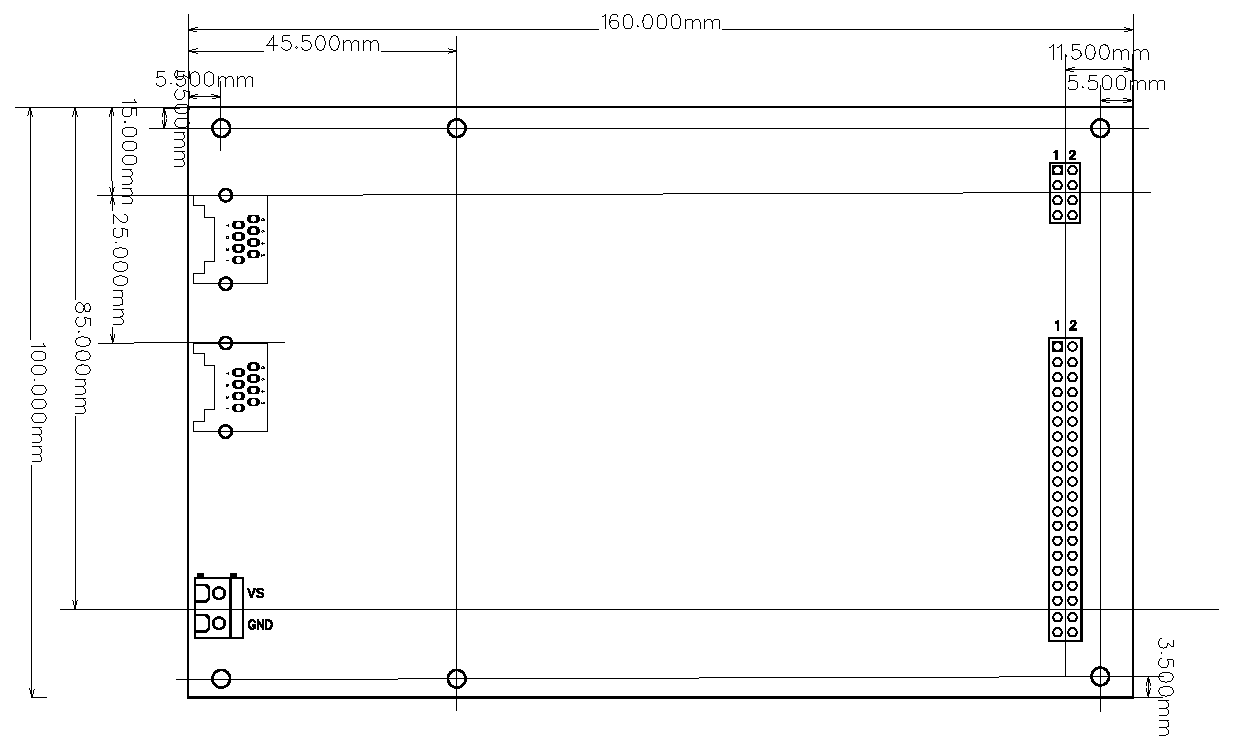
\includegraphics[page=1, scale=0.7]{./Figures/LCS-FP-MAIN-CTRL-10X16.pdf}
    \caption{LCS-FP-MAIN-CTRL-10X16}
    %\label{fig:your-label}
\end{figure}

\FloatBarrier

The mounting holes may look a little odd. As shown in the text to follow, there are extension boards with a form factor of 12cm x 10cm. When are the are mounted on top of the 16cm board, the holes nicely match. 

\section{Extension Boards Footprints}

Next, there are the extension boards. The extension board has the LCS connectors on the left side. The right hand side will typically host the connectors to the layout. These boards can either directly plugged into a controller board or into a bus PCB which hosts controller and more than one extension board. In either case, the extension boards are the same.

\begin{figure}[htbp]
    \centering
    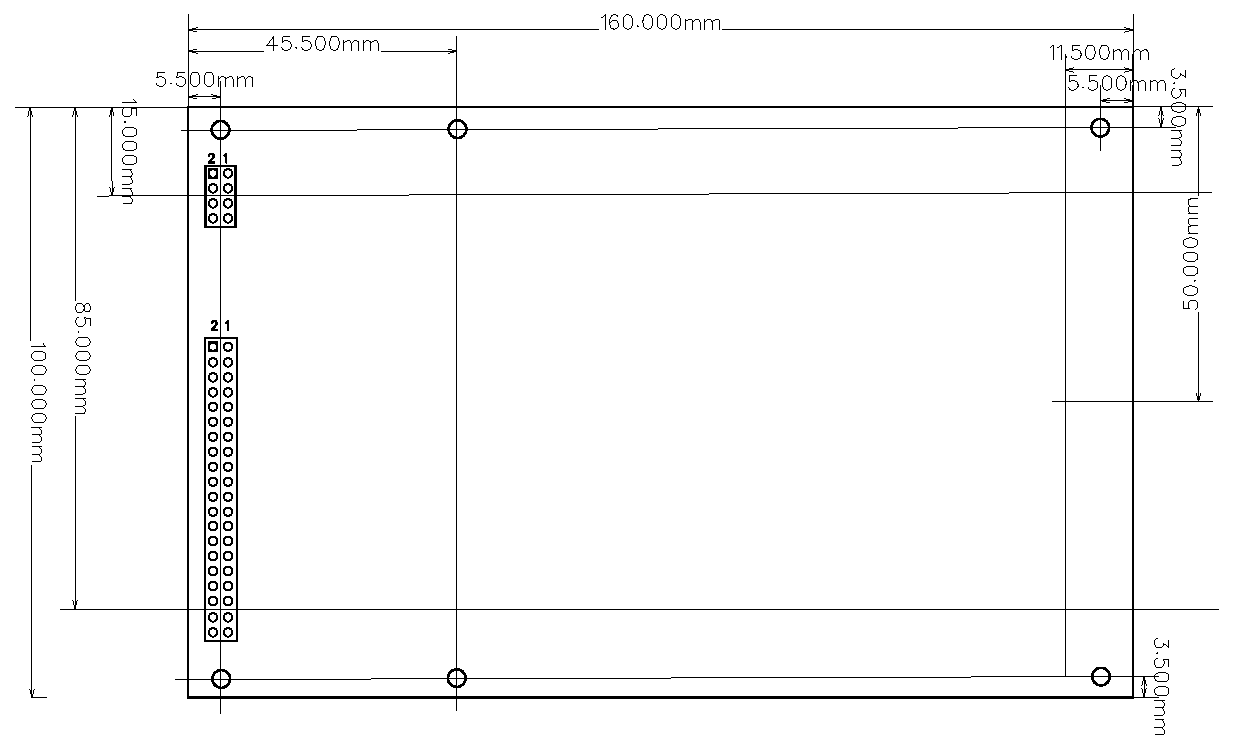
\includegraphics[page=1, scale=0.7]{./Figures/LCS-FP-EXT-L-10X16.pdf}
    \caption{LCS-FP-EXT-R-10X16}
    %\label{fig:your-label}
\end{figure}

\FloatBarrier

In addition to the basic 16cm x 10cm form factor is a set of 12cm x 10cm boards. They have exactly the same layout, except that their length is 12cm instead of 16cm. As always, there could be many more combinations as new boards with different demands are developed. Nevertheless it is important that when connectors are used, that they have the same meaning and are placed at the same location. This is the whole idea of using footprints to ensure this exact fitting.

\section{Pad Numbers}

In EasyEDA, the symbol pads and the PCB pads meet via PAD numbers. Across all symbols and PCBs the numbers assignments are shown in the figure below.

\begin{figure}[htbp]
    \centering
    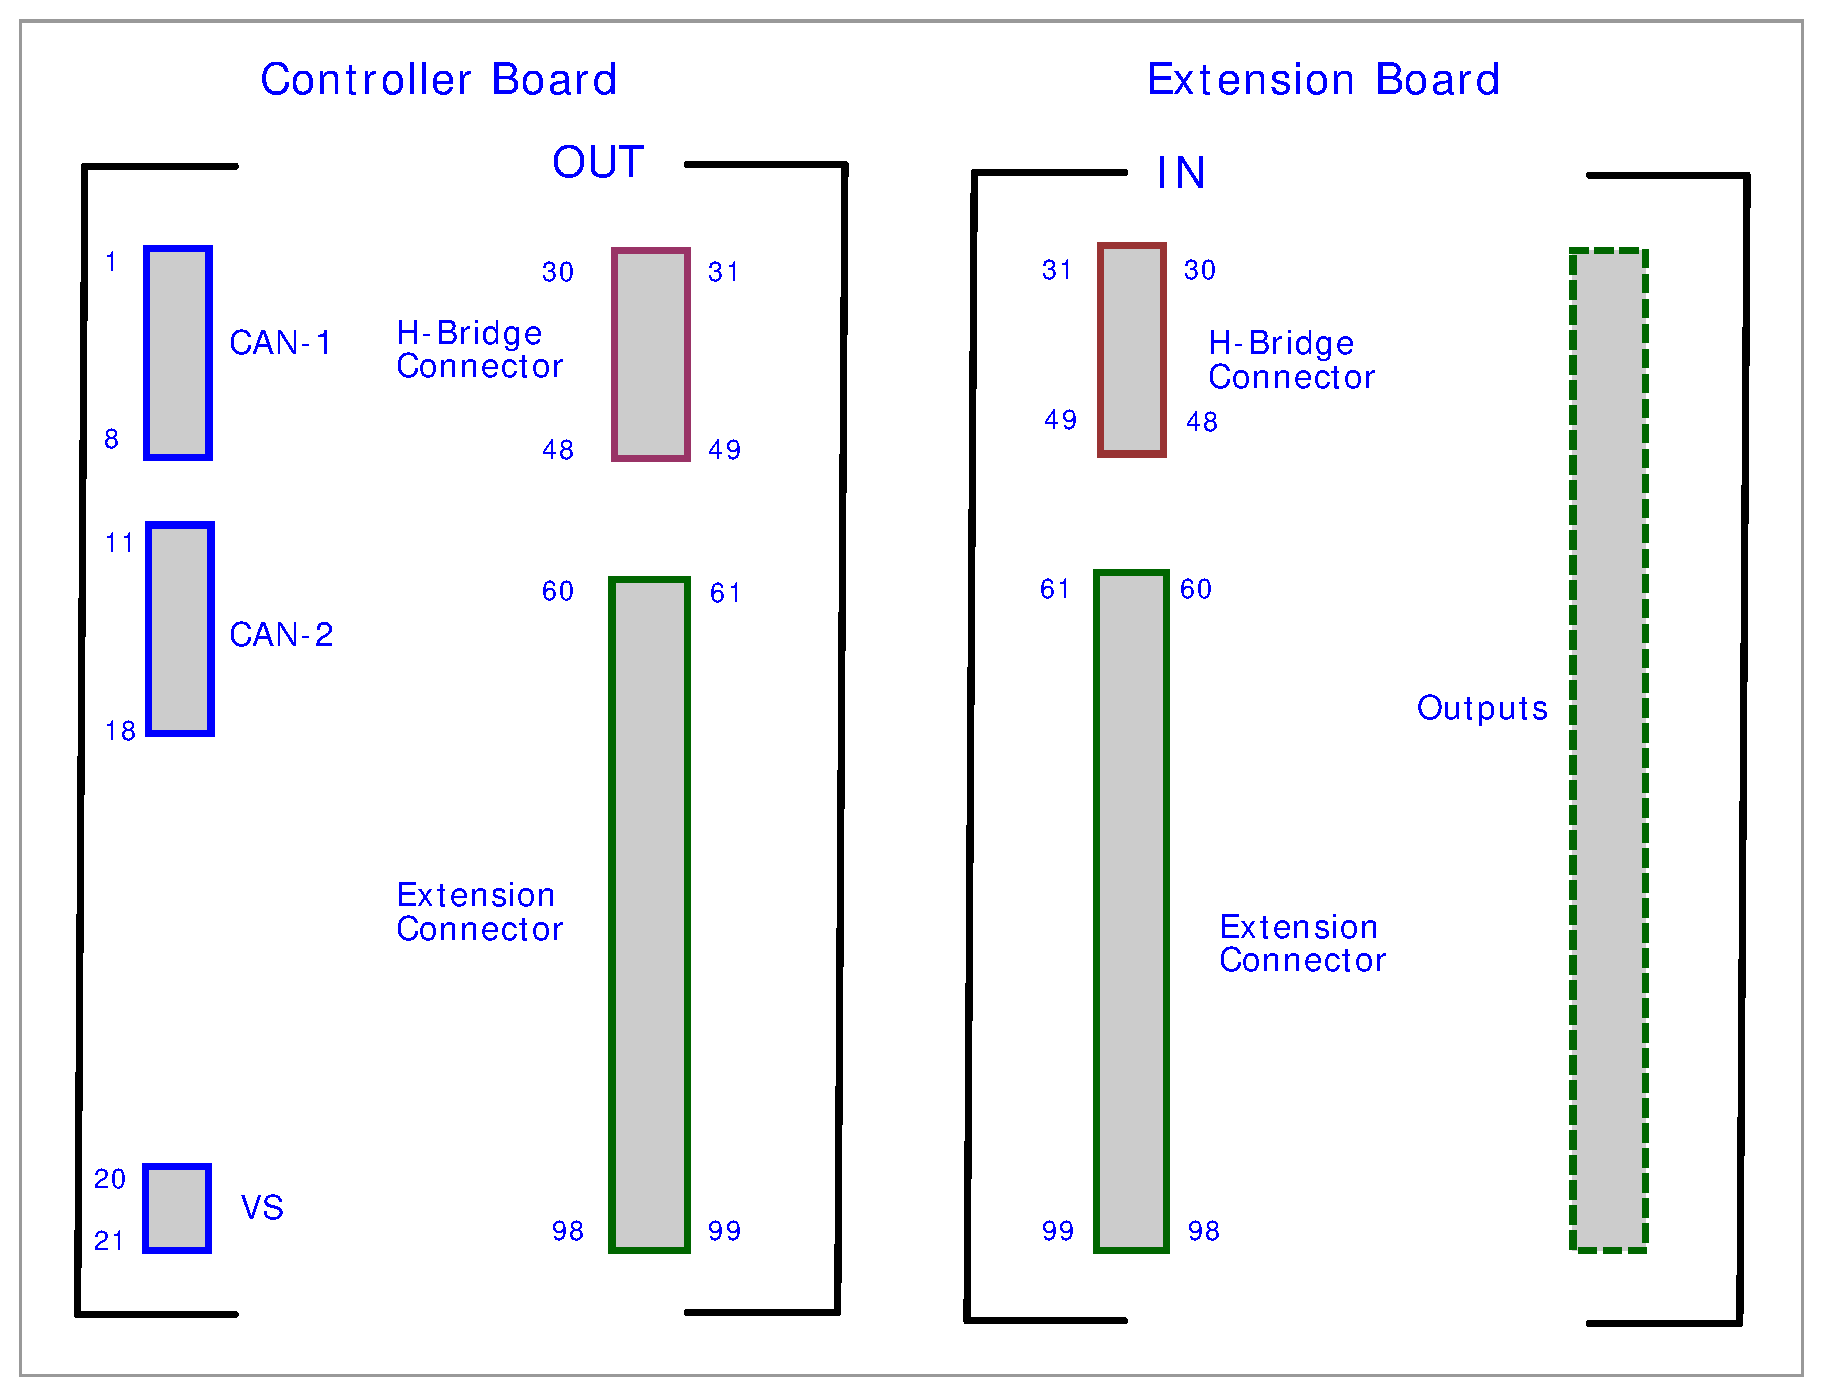
\includegraphics[page=1, scale=0.4]{./Figures/PCB-Connector-Footprint-Pad-Numbers.pdf}
    \caption{PCB-Connector-Footprint-Pad-Numbers}
    %\label{fig:your-label}
\end{figure}

\FloatBarrier

\section{Links}

\begin{table}[!ht]
    \begin{center}
        \caption{...}
        \begin{tabular}{|l|l|p{0.5\textwidth}|}
            \toprule
            \textbf{Tool} & \textbf{Link} & \textbf{Comment} \\
            \midrule
            EasyEDA & http://easyeda.com/de & Design tool for schematics and PCB layouts \\
            \midrule
            JLCPCB & - & PCB board manufactures and parts provider, order from within EasyEDA \\
            \bottomrule
        \end{tabular}
    \end{center}
\end{table}

    \include{appendices/appendix-inspiring-work-and-links} 
    \chapter{Tests}

\section{Schematics}

float barrier command to ensure that text stays close to the picture but no text from after the pciture.

\subsection{part 1}

\begin{figure}[ht]
    \centering
    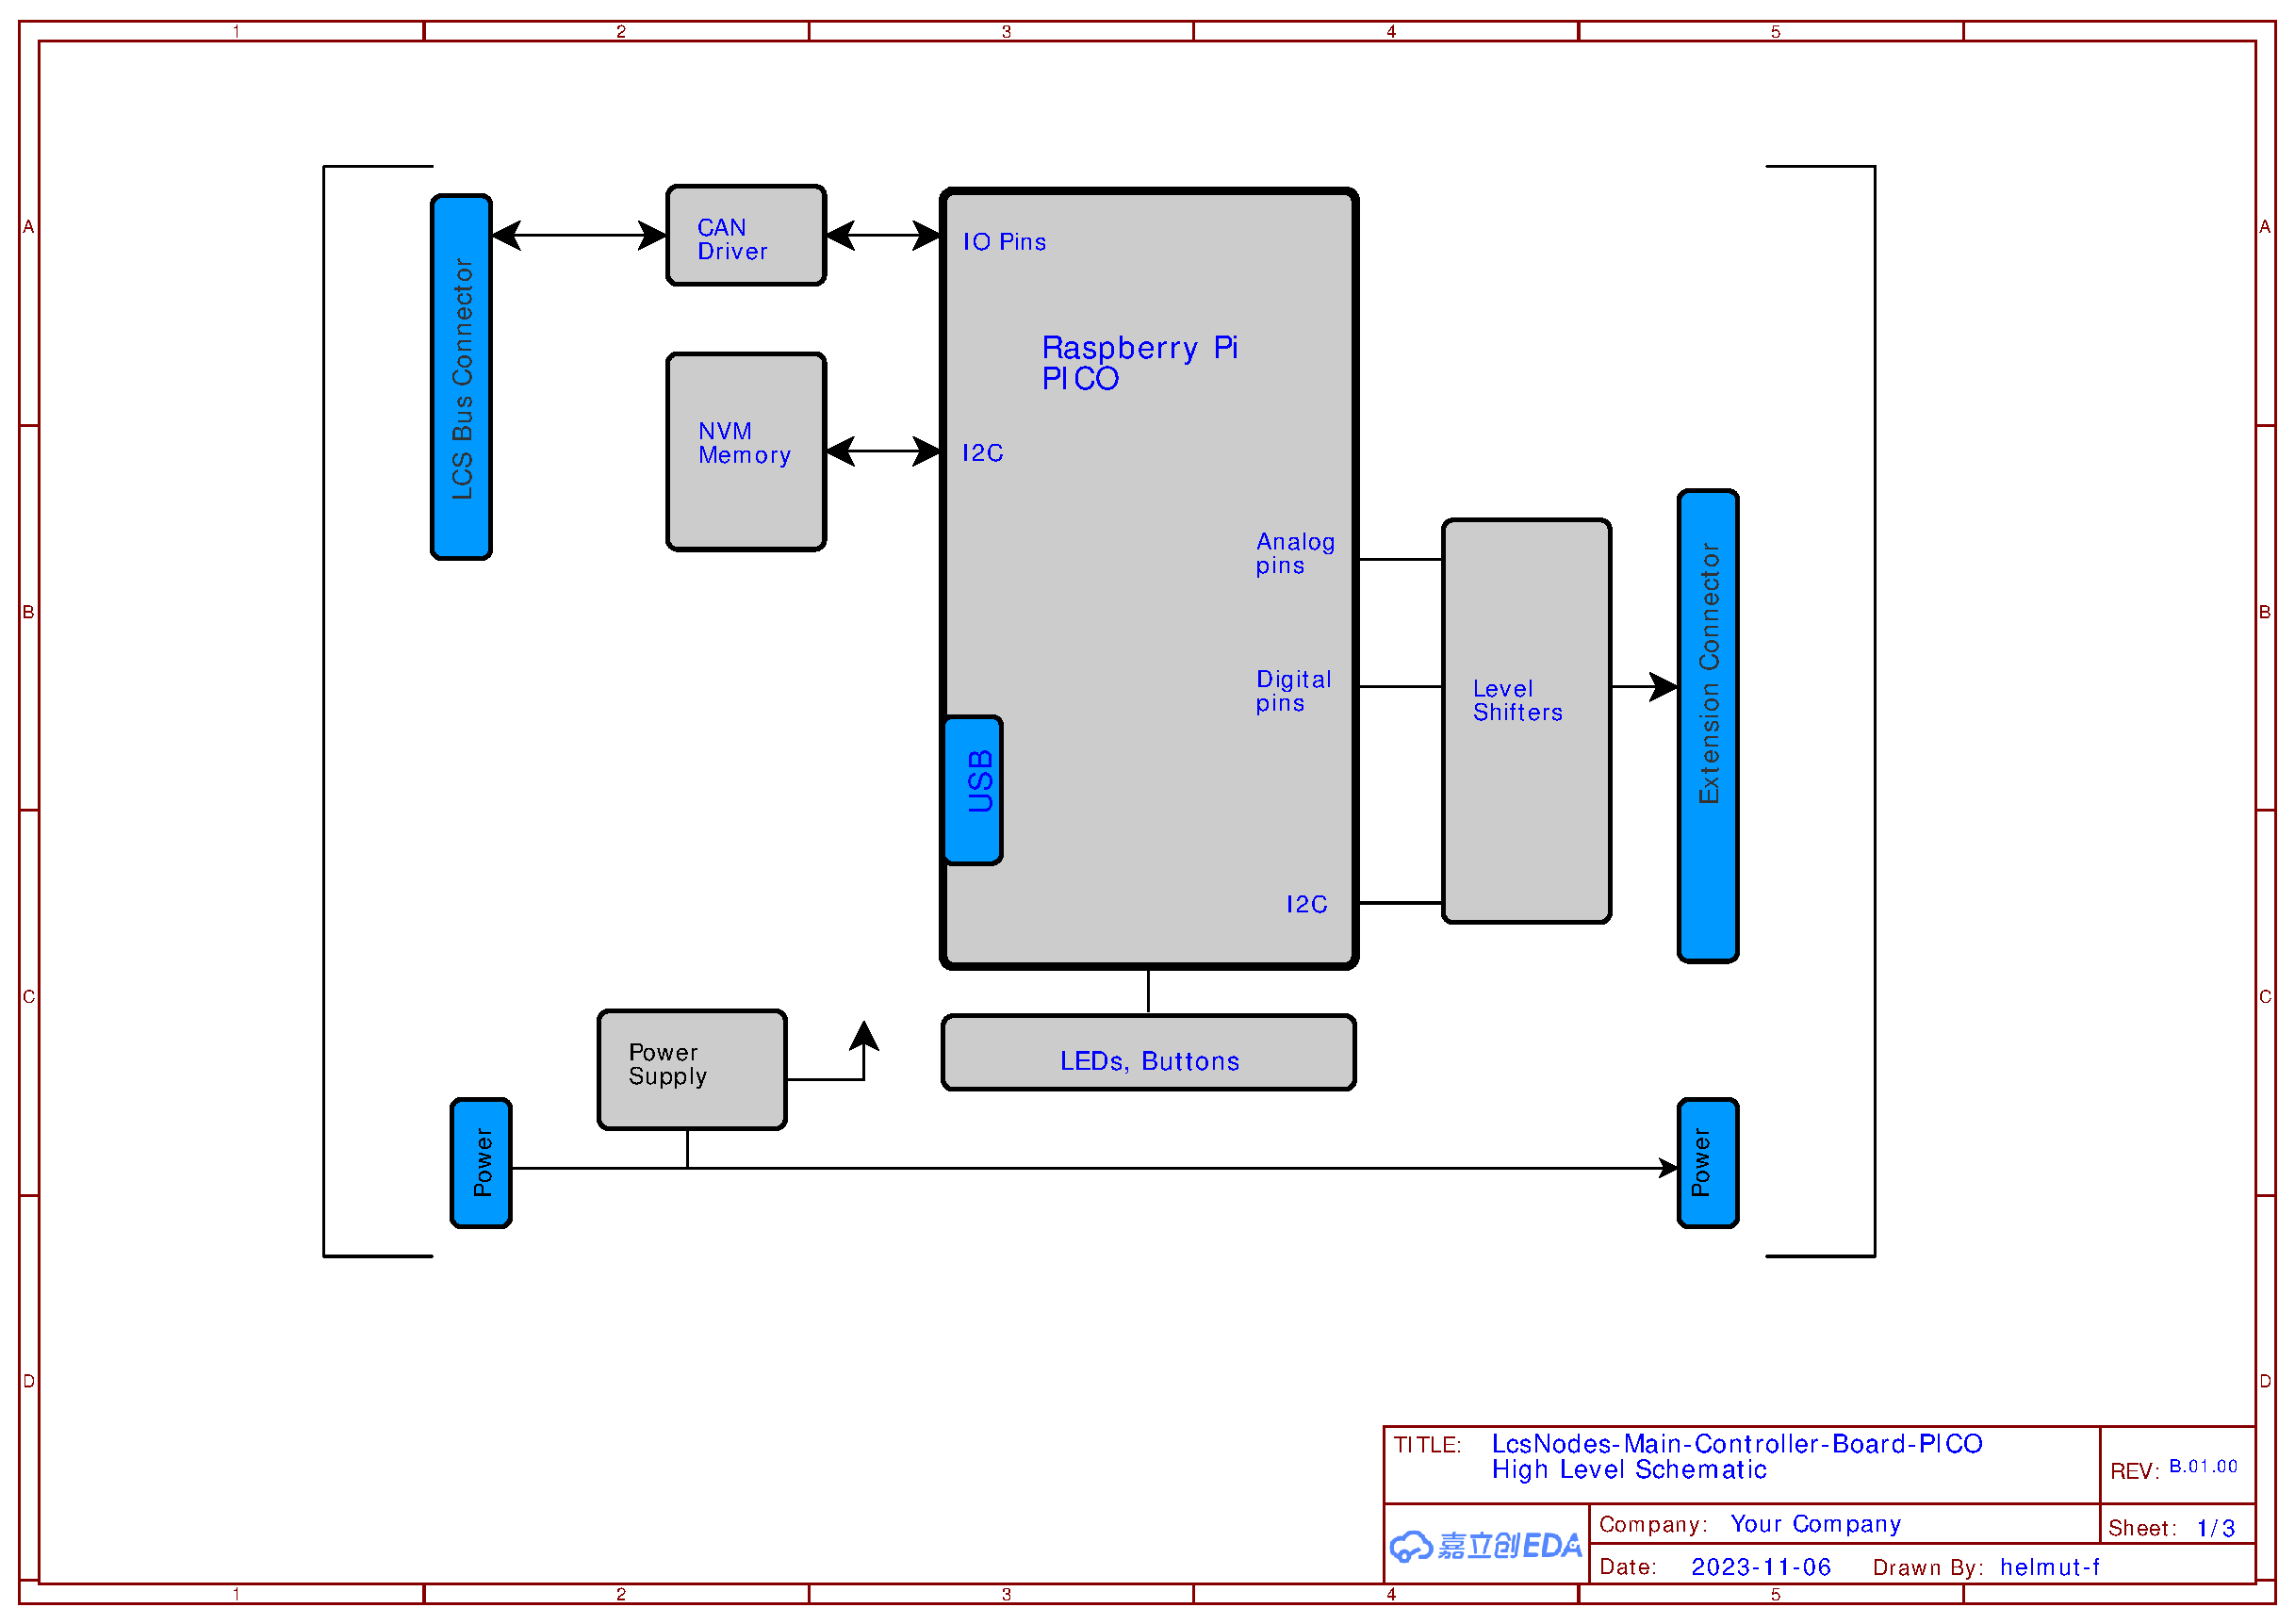
\includegraphics[page=1, width=\textwidth]{./schematics/Schematic_LcsNodes-Main-Controller-Board-B.01.00.pdf}
\end{figure}

\FloatBarrier

\subsection{part 2}
\begin{figure}[ht]
    \centering
    \includegraphics[page=2, width=\textwidth]{./schematics/Schematic_LcsNodes-Main-Controller-Board-B.01.00.pdf}
\end{figure}

\FloatBarrier

\subsection{part 3}
\begin{figure}[ht]
    \centering
    \includegraphics[page=3, width=\textwidth]{./schematics/Schematic_LcsNodes-Main-Controller-Board-B.01.00.pdf}
\end{figure}

\FloatBarrier


\section{Code Snippets}

\lstset{style=listingstyle}
\begin{lstlisting}

    int main( int argc, char **argv ) {

        return( 0 );
    }
    
\end{lstlisting}


\section{Lists}

\subsection{ a simple list}

\begin{itemize}
    \item First bullet point
    \item Second bullet point
    \item Third bullet point
\end{itemize}




    
    % \include{appendices/LCS-Item-Reference}
    % \include{appendices/LCS-Command-Reference}
    % \include{appendices/DCC-PP-Command-Reference}
    % \chapterr{\textit{Appendix n - Runtime Library Routines Reference}}

// ??? \textbf{note} this appendix will not repeat what is documented in the source. This is a battle you cannot win. I have a small utility that takes an augmented C-source include file and makes it a markdown document. 

// ??? \textbf{note} we could just include this file, or keep a reference to it for the utility to include. The result of the utility is a markdown file with all the text in this file and the included files, which is then the base for PDF creation.

// ?? \textbf{note} have a table with all items... 

| Item | purpose | Get | Put | Req |
|:--|:--|:--:|:--:|:--:|
| an item | what it does | X | X | - |
    % ## *Appendix n - Controller Dependent Code Library Routines Reference*

// ??? **note** this appendix will not repeat what is documented in the source. This is a battle you cannot win. I have a small utility that takes an augmented C-source include file and makes it a markdown document. 

// ??? **note** we could just include this file, or keep a reference to it for the utility to include. The result of the utility is a markdown file with
// all the text in this file and the included files, which is then the base for PDF creation.

    % ## *Appendix n - A generic power supply*

Depending on the actual node hardware design, power is implemented in a variety of ways. A small handheld node would certainly draw its power from the LCS bus. A booster has a much higher power consumption requirement. The typical node needs in any case a 5V power, which can for example be drawn from a high power line on the layout. And as with every building block shown so far, there are many ways to Rome.

A power supply for a generic node could draw power from the LCD bus or from an external power line. Furthermore, some LCS nodes need a way to detect a power failure and perform any last second items before power is gone. The following schematic shows a power supply that allows for automatic switching between two inputs. It also features a power fail detection mechanism.


![Schematic_LcsNodes-Building-Block-Generic-Power-Supply.png](./Schematics/Schematic_LcsNodes-Building-Block-Generic-Power-Supply.png )

The right part of the schematic shows how the power input lines are switched depending what is connected. The voltage regulator itself is pretty much standard. Since the power line may have up to 24Volts, a switched regulator is a good choice. The right side features a power fail signal detection output and a capacitor to provide power for the last actions before power done. Naturally the timing depends on the actual power drawn by the board. When a power fail is detected, it is a good idea to immediately turn off power consuming devices and focus on the last items to do before power is gone. A good example is to save the last data items in the non-volatile storage.
    % \include{appendices/appendix-lcs-guidance-computer}
    
    % \iftoggle{includeListings}{ \chapter{Listings test}

Here is a little test how a listing part might be shown ...

\lstset{style=listingstyle}
\lstinputlisting[language=c++]{./listings/main.cpp}
 }
        
    \backmatter    
    
    \printindex         

\end{document}
